\documentclass[11pt]{article}
\usepackage[margin=1in]{geometry}
\usepackage{amsmath,amssymb,amsthm}
\usepackage{booktabs}
\usepackage{longtable}
\usepackage{array}
\usepackage{enumitem}
\usepackage{tikz}
\usetikzlibrary{arrows.meta,calc}
\usepackage[hidelinks]{hyperref}
\setlist{itemsep=1pt,topsep=3pt,parsep=0pt}

\newtheorem{theorem}{Theorem}[section]
\newtheorem{lemma}[theorem]{Lemma}
\newtheorem{proposition}[theorem]{Proposition}
\newtheorem{corollary}[theorem]{Corollary}
\theoremstyle{definition}
\newtheorem{definition}[theorem]{Definition}
\newtheorem{example}[theorem]{Example}
\newtheorem{remark}[theorem]{Remark}

\newcommand{\Q}{\mathbb{Q}}
\newcommand{\Z}{\mathbb{Z}}
\newcommand{\R}{\mathbb{R}}
\newcommand{\F}{\mathbb{F}}
\newcommand{\cO}{\mathcal{O}}
\newcommand{\m}{\mathfrak{m}}
\newcommand{\sg}{\sigma}
\newcommand{\Area}{\operatorname{Area}}
\newcommand{\tL}[1]{\texttt{#1}}
\newcommand{\ar}[1]{[#1]}
\tikzset{
  vec/.style={-{Stealth[length=2.4mm]},thick},
  pt/.style={circle,fill=black,inner sep=1.1pt},
  lab/.style={font=\small}
}

\title{Monsky's theorem and Stein's conjecture:\\
a proof by merging parallel side vectors}
\author{Luka Horjak\thanks{Faculty of Mathematics and Physics, University of Ljubljana, Slovenia}
\and Matevž Miščič\footnotemark[1]\thanks{Institute of Mathematics, Physics and Mechanics (IMFM), Ljubljana, Slovenia}
\and Job Petrovčič\footnotemark[1]
\and Luka Ponikvar\footnotemark[1]}
\date{Mathathon, Round 1 --- problem 067 --- November 2026\\
\small Lean project and scripts: \url{https://github.com/MatevzMiscic/MathathonSubmission}, tag \texttt{submission}}

\begin{document}
\sloppy
\maketitle

\begin{abstract}
A polygon is \emph{special} if, for every direction, its oriented boundary edges in that direction
sum to zero. Stein conjectured (2000) that a special polygon cannot be cut into an odd number of
triangles of equal area; for the square this is Monsky's theorem (1970). The most general result we
found in the literature is Rudenko's: the conjecture holds when all triangle vertices have rational
coordinates.

We present a \textbf{proof for arbitrary real coordinates}. The main statement is an
inequality that holds for \emph{every} valuation $v$ on a field containing the coordinates of the
triangle vertices: for a dissection of a special polygon $P$ into triangles $T_1,\dots,T_n$,
\[ v(2\Area P)\ \ge\ v(2)+\min_iv(2\Area T_i). \]
Stein's conjecture follows by choosing $v$ with $v(2)>0$. The proof uses no colouring of the plane
and no Sperner lemma; it uses a valuation on the countable field generated by the coordinates.
Valuations remain essential, but only through their three axioms. The
ingredients are: closed sequences of side vectors with three moves (join, swap, add); a geometric
\emph{balance} lemma; and one induction (``merge a longest side vector with an equally long
parallel one''). The factor $2$ appears in one place: exchanging two neighbouring steps of a closed
path changes the enclosed area by a parallelogram, which is twice a triangle.

\textbf{Status.} The main result has not been peer-reviewed. To the best of our knowledge it has not
been shown before. The Key Proposition, Stein's conjecture and Monsky's theorem are verified in Lean
(Section~\ref{sec:lean}). The proofs, the Lean code, the computations and this text were
produced by AI agents (Section~\ref{sec:ai}).
\end{abstract}

\tableofcontents

%=====================================================================
\section{The problem and the result}\label{sec:intro}

\subsection{Definitions}

\paragraph{Polygons.} A \emph{simple closed polygonal curve} is given by points
$p_1,\dots,p_m\in\R^2$ ($m\ge3$), pairwise distinct, such that two of the segments
$[p_k,p_{k+1}]$ (indices modulo $m$) meet only if they are consecutive, and then only in their
common end point. The \emph{polygon} $P$ bounded by the curve $C$ is the union of $C$ and of the set
of points of $\R^2\setminus C$ around which $C$ has non-zero winding number. By the Jordan curve
theorem for polygons, $P$ is the closure of the bounded component of $\R^2\setminus C$, a point off
$C$ lies in $P$ if and only if a ray from it that avoids the vertices crosses $C$ an odd number of
times, and $\Area P$ is given by the shoelace formula; these equivalences are Lean-verified
(Section~\ref{sec:lean}). The proof uses only the two facts about $P$ stated in
Appendix~\ref{sec:proofB}. The points $p_k$ are the \emph{vertices}. We number them so that $P$
lies on the left of each oriented segment $p_k\to p_{k+1}$ (counter-clockwise order; that one of
the two orders has this property is part of Proposition~\ref{fact:P}); these oriented segments are the
\emph{edges} of $P$, and $p_{k+1}-p_k$ is an \emph{edge vector}.

\paragraph{Dissections.} A \emph{triangle} is the convex hull of three non-collinear points. A
\emph{dissection} of $P$ is a finite set of triangles $T_1,\dots,T_n$ with union $P$ and pairwise
disjoint interiors. The vertices may be arbitrary real points, and a vertex of one triangle may lie
in the interior of a side of another (a \emph{T-junction}). \emph{Area} is Lebesgue measure. A
dissection is an \emph{equidissection} if all $T_i$ have the same area.

\begin{definition}[{Stein \cite[p.~141]{Ste00}; wording of \cite{Rud}}]\label{def:special}
$P$ is \emph{special} if for every line $D$ through $0$, the edge vectors of $P$ parallel to $D$
sum to $0$.
\end{definition}

The definition does not depend on the orientation, and it does not change if a point in the
interior of an edge is declared to be a vertex.

\begin{lemma}[examples]\label{lem:examples}
\begin{enumerate}[label=(\alph*)]
\item A polygon whose edges have only two directions is special. In particular parallelograms are
special, and so are polyominoes (polygons that are unions of unit squares of the grid $\Z^2$).
\item A centrally symmetric polygon is special.
\item The image of a special polygon under an invertible affine map is special.
\end{enumerate}
\end{lemma}

\begin{proof}
(a) The sum of all edge vectors of a closed curve is $0$. If $s_1$ and $s_2$ are the sums of the
edge vectors in the two directions, then $s_1+s_2=0$ with $s_1,s_2$ on two different lines through
$0$, so $s_1=s_2=0$. (b) Let $\rho(x)=2c-x$ be the point reflection with $\rho(P)=P$; we may assume
that the set of vertices is invariant under $\rho$ (add vertices in the interior of edges if
necessary). Since $\rho(\partial P)=\partial P$ and the vertex set is invariant, $\rho$ maps the segment
of the curve between two consecutive vertices to such a segment; and since $\rho$ is a rotation,
it maps each edge $E$, with $P$ on its left, to an edge $\rho(E)$, with $P$ on its left, and the edge vector of $\rho(E)$ is minus that of $E$. In
particular $\rho(E)\ne E$. So the edges in a given direction fall into pairs $\{E,\rho(E)\}$ with
opposite edge vectors. (c) The linear part of the map sends edge vectors to edge vectors and
parallel classes to parallel classes; if it reverses the orientation, all edge vectors change sign.
\end{proof}

A trapezoid that is not a parallelogram is not special, and ``special'' cannot simply be dropped:
the trapezoid with vertices $(0,0),(2,0),(1,1),(0,1)$ has horizontal edge vectors $(2,0)$ and
$(-1,0)$, with sum $(1,0)\ne0$, and it has an equidissection into three triangles of area
$\tfrac12$, with vertices $(0,0),(1,0),(0,1)$; $(1,0),(1,1),(0,1)$; $(1,0),(2,0),(1,1)$
(Figure~\ref{fig:special}).

\begin{figure}[ht]
\centering
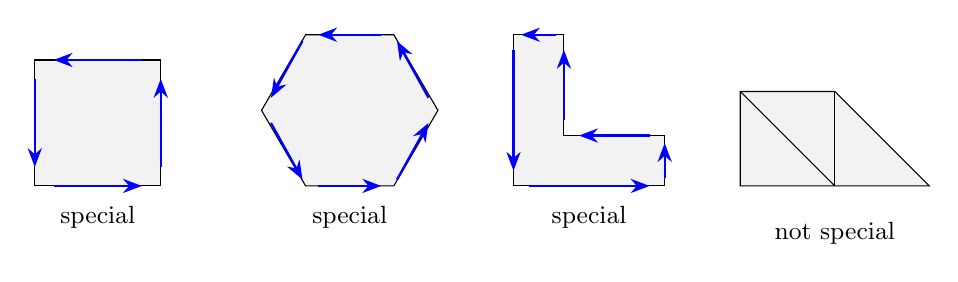
\begin{tikzpicture}[scale=0.8]
\begin{scope}
\draw[fill=gray!10] (0,0)--(2,0)--(2,2)--(0,2)--cycle;
\draw[vec,blue] (0.3,0)--(1.7,0); \draw[vec,blue] (2,0.3)--(2,1.7);
\draw[vec,blue] (1.7,2)--(0.3,2); \draw[vec,blue] (0,1.7)--(0,0.3);
\node[lab] at (1,-0.5) {special};
\end{scope}
\begin{scope}[xshift=3.6cm]
\draw[fill=gray!10] (0.7,0)--(2.1,0)--(2.8,1.2)--(2.1,2.4)--(0.7,2.4)--(0,1.2)--cycle;
\draw[vec,blue] (0.9,0)--(1.9,0); \draw[vec,blue] (2.15,0.1)--(2.65,1.0);
\draw[vec,blue] (2.65,1.4)--(2.15,2.3); \draw[vec,blue] (1.9,2.4)--(0.9,2.4);
\draw[vec,blue] (0.65,2.3)--(0.15,1.4); \draw[vec,blue] (0.15,1.0)--(0.65,0.1);
\node[lab] at (1.4,-0.5) {special};
\end{scope}
\begin{scope}[xshift=7.6cm,scale=0.8]
\draw[fill=gray!10] (0,0)--(3,0)--(3,1)--(1,1)--(1,3)--(0,3)--cycle;
\draw[vec,blue] (0.3,0)--(2.7,0); \draw[vec,blue] (3,0.15)--(3,0.85); \draw[vec,blue] (2.7,1)--(1.3,1);
\draw[vec,blue] (1,1.3)--(1,2.7); \draw[vec,blue] (0.85,3)--(0.15,3); \draw[vec,blue] (0,2.7)--(0,0.3);
\node[lab] at (1.5,-0.62) {special};
\end{scope}
\begin{scope}[xshift=11.2cm,scale=1.5]
\draw[fill=gray!10] (0,0)--(2,0)--(1,1)--(0,1)--cycle;
\draw (1,0)--(0,1); \draw (1,0)--(1,1);
\node[lab,align=center] at (1,-0.5) {not special};
\end{scope}
\end{tikzpicture}
\caption{A square, a centrally symmetric hexagon and an L-shaped polyomino, each with its
edge vectors drawn as arrows; in each direction the arrows cancel. The trapezoid with parallel
sides $2$ and $1$ is not special, and the two segments drawn in it cut it into three triangles of
area $\tfrac12$.}\label{fig:special}
\end{figure}

\subsection{The result}

Throughout, $\det(a,b)=a_1b_2-a_2b_1$ for $a,b\in K^2$. Valuations are defined in
Section~\ref{sec:val}.

\begin{proposition}[Key Proposition; Lean-verified in the form of Section~\ref{sec:lean}]\label{thm:main}
Let $T_1,\dots,T_n$ be a dissection of a special polygon $P$, let $K\subset\R$ be a field containing
the coordinates of all vertices of the triangles, and let $v$ be any valuation on $K$. Then
$2\Area P\in K$, $2\Area T_i\in K$, and
\[ v(2\Area P)\ \ge\ v(2)+\min_iv(2\Area T_i). \]
\end{proposition}

\begin{corollary}[Stein's conjecture; Monsky's theorem for the square; same status]\label{cor:stein}
A special polygon has no equidissection into an odd number of triangles.
\end{corollary}

Both are proved in Section~\ref{sec:end}. The proof of Proposition~\ref{thm:main} consists of a
geometric lemma (Lemma~\ref{lem:B}, Section~\ref{sec:balance}) and an algebraic theorem about
families of closed sequences of vectors (Theorem~\ref{thm:M}, Section~\ref{sec:core}).
Appendix~\ref{sec:expert} repeats the whole proof on one page for a reader who knows valuation
rings. How each claim is supported is recorded once, in Table~\ref{tab:support}; the limitations
are collected in Section~\ref{sec:limits}.

\subsection{Known results}\label{sec:known}

\begin{itemize}
\item \textbf{The square} \cite{Mon70}: Monsky's theorem. According to \cite[Section 1]{Rud12}, the
proof ``is based on two key ideas: the Sperner's Lemma and the coloring of the plane in three colors
based on a $2$-adic valuation''; the problem statement says the same, and names the exposition
\cite{AZ}. Monsky states and proves more \cite[pp.~161--162]{Mon70}: if $[0,1]^2$ is divided
into $m$ triangles of areas $a_1,\dots,a_m$, then ``there is a polynomial $f$ with integer
co-efficients such that $f(a_1,\dots,a_m)=1/2$''. His proof has a combinatorial lemma of Sperner
type for a region bounded by a simple closed polygon (stated with ``basic segments'', so that
T-junctions are allowed) and a colouring of the plane in three sets by an ultranorm on $\R$ with
$\|2\|<1$: a line meets at most two of the sets, and a triangle with vertices in all three has an
area of norm $>1$ \cite[pp.~162--163]{Mon70}. The exposition \cite[Chapter 22]{AZ} gives the
argument ``in a version due to Hendrik Lenstra'' \cite[p.~157]{AZ}, for a valuation with values in
an ordered abelian group, and proves the existence of such a valuation on $\R$ with Zorn's lemma.
The colouring and its two properties are also in \cite[Section 2, Lemma 1]{Rud12}.
\item \textbf{Centrally symmetric polygons} \cite{Mon90}: proved by Monsky in 1990 (problem
statement). His theorem is for any set $S=-S$ in $\R^2$ that is a finite union of non-overlapping
triangles, with arbitrary real vertices: if the areas are equal, the number of triangles is even
\cite[Theorem 3.8]{Mon90}; and if $S$ has area $2$ and the areas are $a_i$, then $1$ is a
polynomial in the $a_i$ with integer coefficients and zero constant term \cite[Theorem
3.10]{Mon90}. The proof works in the group of closed chains of segments modulo chains supported in
a line, with a valuation ring $(\cO,\m)$, $2\in\m$, that is ``almost discrete''
\cite[Definition 3.5]{Mon90}, tricolourings, and the homology of the group of order two generated
by the reflection in the origin. According to \cite[Section 1]{Rud12} the proof is ``based on the same idea of
$3$-coloring'' and ``uses a non-trivial homological technique''; \cite[Introduction]{Rud} calls it
``a much more difficult result''.
\item \textbf{The conjecture.} Stein \cite{Ste00} conjectured that the same holds for a larger
class of polygons. The two papers of Rudenko state the class differently: \cite{Rud12} for
\emph{balanced} polygons (the edges ``can be divided into pairs so that in each pair edges are
parallel, equal in length and have opposite orientation''), \cite{Rud} for \emph{special} polygons
as in Definition~\ref{def:special}. A balanced polygon is special, and a special polygon becomes
balanced after subdividing edges (Section~\ref{sec:limits}, item~3). Stein's own formulation
\cite[p.~141]{Ste00} is that of Definition~\ref{def:special}, for a ``simply connected polygon''
with oriented boundary, and the conjecture reads: ``A special polygon cannot be cut into an odd
number of triangles of equal areas.'' In the same paper he proves it for special polygons with at
most six sides, with real vertices (his Theorems 1 and 2, by Monsky's colouring for a $2$-adic
valuation on $\R$ after suitable affine maps), and says without details that similar arguments
settle ``several families of special polygons with more than six sides'' \cite[p.~145]{Ste00}.
\item \textbf{Polyominoes.} Stein \cite[p.~256]{Ste99} proved that a polyomino consisting of an
odd number of unit squares has no odd equidissection, and conjectured the same for all polyominoes
(his Conjecture 1) and for all polygons bounded by lines parallel to the axes (his Conjecture 2).
Praton \cite[Theorem 6]{Pra} proved Conjecture 1: no polyomino (a finite union of unit squares of
the grid, not necessarily connected) has an odd equidissection. Both proofs use Monsky's colouring
after maps $(x,y)\mapsto(x/2^r,y/2^s)$ and translations, and a count of labelled edges on the
boundary \cite[Chapter 5]{SS}; Praton adds a divisibility argument for integer matrices that count
the squares. Neither statement restricts the vertices of the triangles; both papers define the
labelling for points with rational coordinates and refer to \cite{Mon70,SS} for the lemma they use,
which \cite[p.~118]{SS} states for a valuation on $\R$.
\item \textbf{Lattice polygons} \cite{Rud12}: a balanced polygon with integer vertices and odd
integer area has no odd equidissection. The proof combines Monsky's colouring, applied after three
affine maps, with a homology class of the boundary in a graph on $(\Z/2)^2$; to treat a balanced
boundary, the side vectors of a closed broken line are permuted, and a transposition of two
consecutive side vectors changes the area by a parallelogram; the permutation is chosen so that
paired opposite sides become consecutive, and then they cancel \cite[Section 5, proof of Lemma
5]{Rud12}. So \cite{Rud12} already contains, for the boundary of a balanced polygon, the pattern
``move parallel vectors next to each other by transpositions, pay parallelograms, cancel'' of
Steps~3 and~4 of our Theorem~\ref{thm:M}.
\item \textbf{Rational coordinates} \cite{Rud}: Rudenko's Theorem~2 states that a special polygon
cannot be dissected into an odd number of triangles of equal area ``in such a way that all
coordinates of the vertices of the triangles in the dissection are rational numbers''. It is derived
(his Section~3) from his Theorem~1: in a finite trivalent graph with a $\Q^2$-valued flow, the
number of vertices of minimal weight is even, where the weight of a vertex is the $2$-adic
valuation of the determinant of two of the three flow vectors at it. The graph is built from the
dissection (triangles are vertices, with extra degenerate triangles at T-junctions; boundary sides
are paired using specialness), and the flow assigns to an edge the side vector of the triangle. The
proof of Theorem~1 (his Section~2) uses lattices over $\Z_{(2)}$, the residue field $\F_2$, and a
minimal counterexample in which the flow is modified along cycles of ``odd'' edges (his Lemmas~3--5).
\end{itemize}

\textbf{Attribution to Rudenko, and what we believe is new.} \emph{From \cite{Rud}:} recording a
dissection by the side vectors of its triangles and measuring the determinants of pairs of side
vectors by a valuation; this is the starting point of this report. \emph{From \cite{Rud12}:}
rearranging the side vectors of one closed path by transpositions, at the cost of parallelograms,
until opposite vectors are adjacent and cancel. \emph{Ours, as far as we know:} applying this to
the family of all triangle sequences at once (Join); merging two entries that are parallel and
equally long but not necessarily opposite (Add of $u$ and $tu$ with $v(t)=0$); the choice of a
longest entry and Lemma~\ref{lem:T}, which keep flatness under Join; and the resulting statement
(Theorem~\ref{thm:M}) for an arbitrary field and an arbitrary valuation, with a sum in place of a
count, which implies Rudenko's Theorem~1 (Remark~\ref{rem:rud}) and gives the case of real
coordinates. Monsky's proof for centrally symmetric regions \cite{Mon90} also works with closed
chains of segments and with a valuation ring containing $2$ in its maximal ideal, in an arbitrary
field of characteristic $0$; it uses colourings, the reflection in the origin and a discreteness
condition, and we found no merging step in it. The version of \cite{Rud}
dated May 2025 still states the rational case only, and a literature search (Section~\ref{sec:limits},
item~2) found no proof of the real case; for real coordinates, the sources we read cover
centrally symmetric regions \cite{Mon90}, polyominoes \cite{Ste99,Pra} and special polygons with
at most six sides \cite{Ste00}. This is not a proof of priority, and we do not claim one.

%=====================================================================
\section{Motivation: why previous results are unsatisfactory}\label{sec:motivation}

The problem statement says of the existing proofs that they ``are short but non-constructive and
unintuitive'', and asks for ``a valuation-light or visual proof and clarity on which special polygons
known methods cover''. We sought a more geometric proof that does not rely on abstract machinery.
Two points make the existing proofs unsatisfactory.

\begin{enumerate}
\item \textbf{Heavy machinery.} Monsky's proof \cite{Mon70} extends the $2$-adic valuation to $\R$,
colours the plane with three colours by it, and applies a lemma of Sperner type. The later proofs
add more: homology of a group of closed chains and ``almost discrete'' valuation rings
\cite{Mon90}, flows on trivalent graphs, lattices over $\Z_{(2)}$ and the residue field $\F_2$
\cite{Rud}. Our proof uses side vectors, determinants and one valuation, through its three axioms
only. There is no colouring, no Sperner lemma, no homology and no flows on graphs. The polygon enters through
one geometric lemma (balance), the same for all special polygons, and the factor $2$ comes from one
visible fact: exchanging two neighbouring steps $p,q$ of a closed path changes the enclosed area by
the parallelogram spanned by $p$ and $q$ (Lemma~\ref{lem:moves}(b), Figure~\ref{fig:moves}), which
for two sides of a triangle is twice the triangle.
\item \textbf{No full generality.} Previous works prove only special cases, each under a specific
assumption on the polygon or its coordinates: the square \cite{Mon70}, central symmetry \cite{Mon90},
polyominoes \cite{Ste99,Pra}, at most six sides \cite{Ste00}, integer vertices and odd area
\cite{Rud12}, or rational coordinates \cite{Rud} (Table~\ref{tab:coverage}). Our proof assumes only
that the polygon is special, which covers all the cases above.
\end{enumerate}

\textbf{What ``valuation-light'' means here.} The proof is free of colourings and of Sperner's
lemma. It is not free of valuations: a valuation with $v(2)>0$ on the coordinate field, possibly
non-discrete, is essential, and its existence (Lemma~\ref{lem:V}) is not effective. As in Monsky's
proof, which ``is carried out in the field generated by the coordinates of the vertices''
\cite[p.~164]{Mon70}, this existence is the only non-constructive step. For countable fields we
obtain it without Zorn's lemma. What is light is the use: only the three axioms, no residue field,
no completion. Unlike Rudenko's count of triangles of minimal valuation, which relies on the residue
field $\F_2$ and can fail over $\Q(\sqrt5)$ (Example~\ref{ex:fan}), our statement is a sum that holds
for every valuation.

%=====================================================================
\section{The arithmetic input: a valuation ring with \texorpdfstring{$\tfrac12\notin\cO$}{1/2 not in O}}\label{sec:val}

A \emph{valuation} on a field $K$ is a map $v\colon K\to\Gamma\cup\{\infty\}$ into a totally ordered
abelian group $\Gamma$ (with $\infty$ larger than every element of $\Gamma$) such that
\begin{itemize}
\item[(V1)] $v(x)=\infty$ if and only if $x=0$;
\item[(V2)] $v(xy)=v(x)+v(y)$;
\item[(V3)] $v(x+y)\ge\min(v(x),v(y))$.
\end{itemize}
Its ring $\cO=\{x:v(x)\ge0\}$ satisfies: $x\in\cO$ or $x^{-1}\in\cO$ for every $x\ne0$. Its maximal
ideal is $\m=\{x:v(x)>0\}$, and its group of units is $\cO^\times=\{x:v(x)=0\}$. Conversely, every
subring $\cO\subseteq K$ such that $x\in\cO$ or $x^{-1}\in\cO$ for all $x\ne0$ is the ring of a
valuation, namely $v\colon K^\times\to K^\times/\cO^\times$ with the order
$v(x)\ge v(y)\iff x/y\in\cO$. We switch freely between the two languages; $v(2)>0$ means
$\tfrac12\notin\cO$.

We use only (V1)--(V3) and their immediate consequences: $v(\pm1)=0$; each set $\{x:v(x)\ge\gamma\}$
is a subgroup of $(K,+)$; and $\m$ is closed under addition. For $K=\Q$ one can take the $2$-adic
valuation $v_2$ (the exponent of $2$ in a rational number).

\begin{lemma}[existence]\label{lem:V}
Every countable field $K$ of characteristic $0$ has a valuation with $v(2)>0$.
\end{lemma}

For arbitrary fields of characteristic $0$ this is a case of the classical theorem that every local
subring of a field is dominated by a valuation ring of that field (Chevalley; see
\cite[Lemma 10.50.2]{Stacks}, whose proof uses Zorn's lemma). We only need countable fields
($K=\Q(\text{coordinates})$), where a standard argument avoids Zorn's lemma. Its proof is in
Appendix~\ref{sec:proofV}.


For a vector $w\in K^2$ put $v(w)=\min(v(w_1),v(w_2))$. We say that $w$ is \emph{at least as long as}
$w'$ if $v(w)\le v(w')$: ``long'' means small valuation. (This is a $v$-adic notion of size and has
nothing to do with Euclidean length. For $v=v_2$ on $\Q$, the longest vectors are those with the
highest power of $2$ in a denominator.) Note that $v(tw)=v(t)+v(w)$ for $t\in K$.

%=====================================================================
\section{Triangles as closed sequences}\label{sec:seq}

For a finite sequence $c=(c_1,\dots,c_r)$ of vectors in $K^2$ put
\[ \sg(c)=\sum_ic_i,\qquad\ar c=\sum_{i<j}\det(c_i,c_j). \]
Call $c$ \emph{closed} if $\sg(c)=0$. (For closed $c$, $\ar c$ is twice the signed area enclosed by
the polygonal path with steps $c_1,\dots,c_r$; this is only motivation and is not used.) Splitting
the pairs $i<j$ of a concatenation $cc'$ according to where $i$ and $j$ lie, and using bilinearity,
\begin{equation}\label{eq:C}
\ar{cc'}=\ar c+\ar{c'}+\det(\sg(c),\sg(c')).
\end{equation}

\begin{lemma}[three moves]\label{lem:moves}
Let $A,B$ be sequences and $p,q$ vectors.
\begin{enumerate}[label=(\alph*)]
\item \emph{Join.} If $x$ and $y$ are closed, then $xy$ is closed and $\ar{xy}=\ar x+\ar y$.
\item \emph{Swap.} $\ar{A\,p\,q\,B}=\ar{A\,q\,p\,B}+2\det(p,q)$: exchanging two neighbouring entries
$p,q$ (with $p$ first) changes the bracket by $-2\det(p,q)$.
\item \emph{Add.} $\ar{A\,p\,q\,B}=\ar{A\,(p+q)\,B}+\det(p,q)$: replacing two neighbouring entries by
their sum changes the bracket by $-\det(p,q)$, which is $0$ if $p$ and $q$ are parallel.
\end{enumerate}
All three moves preserve $\sg$.
\end{lemma}

\begin{proof}
(a) is \eqref{eq:C}. (b) Every other entry stays on the same side of both $p$ and $q$, so only the
term of the pair $\{p,q\}$ changes, from $\det(p,q)$ to $\det(q,p)=-\det(p,q)$. (c) For any earlier
entry $e$ the terms $\det(e,p)+\det(e,q)$ become $\det(e,p+q)$, which is the same by bilinearity;
similarly for a later entry. Only the term $\det(p,q)$ disappears.
\end{proof}

Applying (b) repeatedly: moving an entry $q$ to the left past a block $B$ changes the bracket by
$-2\det(\sg(B),q)$. The identities are elementary; (b), for a single closed broken line, is used
in \cite[proof of Lemma 5]{Rud12}.

\begin{figure}[ht]
\centering
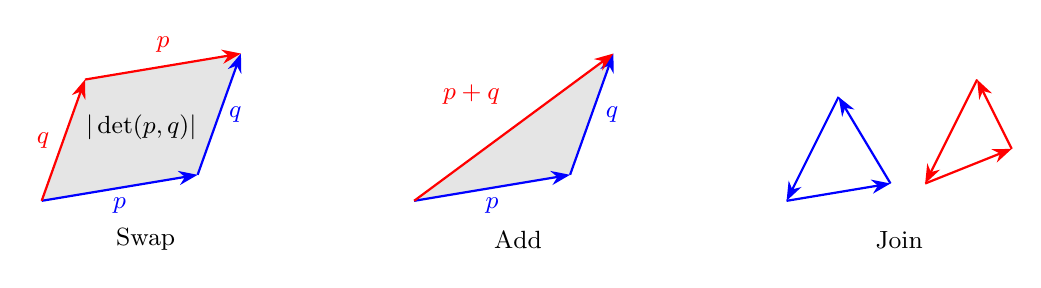
\begin{tikzpicture}[scale=1.1]
\begin{scope}
\coordinate (o) at (0,0); \coordinate (P) at (1.8,0.3); \coordinate (Q) at (0.5,1.4); \coordinate (S) at (2.3,1.7);
\fill[gray!20] (o)--(P)--(S)--(Q)--cycle;
\draw[vec,blue] (o)--(P); \draw[vec,blue] (P)--(S);
\draw[vec,red] (o)--(Q); \draw[vec,red] (Q)--(S);
\node[lab,blue,below] at (0.9,0.15) {$p$}; \node[lab,blue,right] at (2.05,1.0) {$q$};
\node[lab,red,left] at (0.2,0.7) {$q$}; \node[lab,red,above] at (1.4,1.6) {$p$};
\node[lab] at (1.15,0.85) {$|\det(p,q)|$};
\node[lab] at (1.2,-0.45) {Swap};
\end{scope}
\begin{scope}[xshift=4.3cm]
\coordinate (o) at (0,0); \coordinate (P) at (1.8,0.3); \coordinate (E) at (2.3,1.7);
\fill[gray!20] (o)--(P)--(E)--cycle;
\draw[vec,blue] (o)--(P); \draw[vec,blue] (P)--(E); \draw[vec,red] (o)--(E);
\node[lab,blue,below] at (0.9,0.15) {$p$}; \node[lab,blue,right] at (2.1,1.0) {$q$};
\node[lab,red,above left] at (1.1,1.0) {$p+q$};
\node[lab] at (1.2,-0.45) {Add};
\end{scope}
\begin{scope}[xshift=8.6cm]
\draw[vec,blue] (0,0)--(1.2,0.2); \draw[vec,blue] (1.2,0.2)--(0.6,1.2); \draw[vec,blue] (0.6,1.2)--(0,0);
\draw[vec,red] (1.6,0.2)--(2.6,0.6); \draw[vec,red] (2.6,0.6)--(2.2,1.4); \draw[vec,red] (2.2,1.4)--(1.6,0.2);
\node[lab] at (1.3,-0.45) {Join};
\end{scope}
\end{tikzpicture}
\caption{The three moves. Think of a closed sequence as a closed path of arrows drawn head
to tail. \emph{Swap}: two consecutive arrows $p$, then $q$ (blue), are replaced by $q$, then $p$
(red); the old and the new path differ by the parallelogram spanned by $p$ and $q$, of area
$|\det(p,q)|$, so twice the enclosed area changes by $2|\det(p,q)|$. \emph{Add}: two consecutive
arrows are replaced by the single arrow $p+q$; this cuts off the triangle with sides $p,q,p+q$, which
is degenerate when $p$ and $q$ are parallel. \emph{Join}: two closed paths are concatenated into one;
nothing changes because each of them returns to its starting point.}\label{fig:moves}
\end{figure}

\paragraph{Triangles.} For a counter-clockwise triangle $T$ with vertices $p,q,r$, its \emph{side
sequence} is $t=(a,b,c)=(q-p,\ r-q,\ p-r)$. It is closed, and $\det(a,b)=\det(q-p,r-p)=2\Area T$
(the area of a triangle is half the absolute value of this determinant, and the determinant is
positive for counter-clockwise order). Using $c=-a-b$ we get $\det(a,c)=-2\Area T$ and
$\det(b,c)=2\Area T$, so
\begin{equation}\label{eq:tri}
\ar t=2\Area T,\qquad\det(\text{any two different entries of }t)=\pm2\Area T.
\end{equation}

\begin{definition}\label{def:family}
A \emph{family} $F$ is a finite collection of closed sequences (repetitions allowed); $S(F)=\sum_{c\in F}\ar c$. For
$\nu\in\Gamma\cup\{\infty\}$, the family $F$ is \emph{$\nu$-flat} if $v(\det(w,w'))\ge\nu$ for any two
entries $w,w'$ of the \emph{same} sequence. $F$ is \emph{balanced} if, for every line $D$ through
$0$, the entries of $F$ (over all its sequences) lying on $D$ sum to $0$.
\end{definition}

By \eqref{eq:tri}, the side sequences of the triangles of a dissection of $P$ form a $\nu$-flat
family for $\nu=\min_iv(2\Area T_i)$, with $S=\sum_i2\Area T_i=2\Area P$. The last equality is
additivity of area: the triangles are closed sets with pairwise disjoint interiors, and their
boundaries (three segments each) have measure zero, so the measure of the union is the sum of the
measures.

%=====================================================================
\section{Balance: the only geometric input}\label{sec:balance}

\begin{lemma}[Balance]\label{lem:B}
Let $T_1,\dots,T_n$ be a dissection of a polygon $P$, all triangles oriented counter-clockwise. For
every line $D$ through $0$, the sum of the side vectors of the $T_i$ parallel to $D$ equals the sum
of the edge vectors of $P$ parallel to $D$. In particular, if $P$ is special, the family of side
sequences is balanced.
\end{lemma}

\emph{Idea of the proof.} Cut every triangle side and every edge of $P$ at all vertices lying
on it; call the resulting segments \emph{pieces}. A piece inside $P$ is a piece of exactly two
triangle sides, traversed in opposite directions, so its two vectors cancel. A piece on the
boundary of $P$ is a piece of exactly one triangle side and of exactly one edge of $P$, with the
same orientation. Summing over the pieces parallel to $D$ gives the lemma (Figure~\ref{fig:balance}).
The full proof uses two standard facts about simple polygons and is given in
Appendix~\ref{sec:proofB}.

\begin{figure}[ht]
\centering
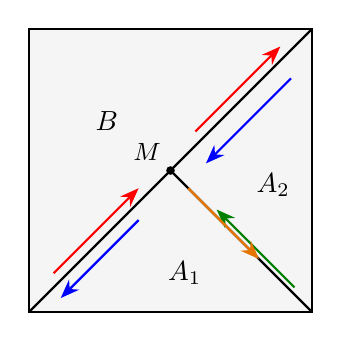
\begin{tikzpicture}[scale=0.9]
\fill[gray!8] (0,0) rectangle (4,4); \draw[thick] (0,0) rectangle (4,4);
\draw[thick] (0,0)--(4,4); \draw[thick] (4,0)--(2,2);
\node[pt] at (2,2) {}; \node[lab,above left] at (2,2) {$M$};
\node at (2.2,0.55) {$A_1$}; \node at (3.45,1.8) {$A_2$}; \node at (1.1,2.7) {$B$};
\draw[vec,red] (0.35,0.55)--(1.55,1.75); \draw[vec,red] (2.35,2.55)--(3.55,3.75);
\draw[vec,blue] (1.55,1.3)--(0.45,0.2); \draw[vec,blue] (3.7,3.3)--(2.5,2.1);
\draw[vec,green!50!black] (3.75,0.35)--(2.65,1.45); \draw[vec,orange!90!black] (2.25,1.75)--(3.25,0.75);
\end{tikzpicture}
\caption{A T-junction. The square $[0,4]^2$ is cut by the diagonal from $(0,0)$ to $(4,4)$,
and the lower right half is cut further by the segment from $(4,0)$ to the midpoint $M=(2,2)$ of the
diagonal. There are three triangles: $B$ above the diagonal, and $A_1$, $A_2$ below it. The side of
$B$ along the diagonal is cut at $M$ into two pieces. On the piece from $(0,0)$ to $M$ the triangles
$B$ and $A_1$ run in opposite directions; on the piece from $M$ to $(4,4)$ the triangles $B$ and
$A_2$ do. The segment from $M$ to $(4,0)$ is one piece, shared by $A_1$ and $A_2$ in opposite
directions. The pieces on the four edges of the square each belong to one triangle.}\label{fig:balance}
\end{figure}

%=====================================================================
\section{The algebraic core}\label{sec:core}

In this section $K$ is any field with a valuation $v$.

\begin{lemma}\label{lem:T}
Let $u,w,w'\in K^2$ with $u\ne0$, $v(u)\le v(w)$ and $v(u)\le v(w')$. Then
\[ v(\det(w,w'))\ \ge\ \min\bigl(v(\det(u,w)),\,v(\det(u,w'))\bigr). \]
\end{lemma}

\begin{proof}
Exchanging the two coordinates if necessary (this changes all determinants by a sign), we may assume
$v(u_1)=v(u)$; in particular $u_1\ne0$. Expanding both sides shows
\[ u_1\det(w,w')=w_1\det(u,w')-w_1'\det(u,w). \]
Divide by $u_1$: the coefficients $w_1/u_1$ and $w_1'/u_1$ have valuation $\ge0$. Apply (V2) and
(V3).
\end{proof}

The identity in the proof is Cramer's rule in the plane. The hypothesis on $u$ is necessary: for
$v=v_2$, $u=(2,0)$, $w=(1,1)$, $w'=(0,1)$ we have $v(\det(u,w))=v(\det(u,w'))=1$ but
$v(\det(w,w'))=0$.

\begin{theorem}\label{thm:M}
If $F$ is a $\nu$-flat balanced family, then $v(S(F))\ge v(2)+\nu$.
\end{theorem}

\begin{proof}
Let $I=\{x\in K:v(x)\ge v(2)+\nu\}$, an additive subgroup of $K$. We use induction on the number of
entries of $F$. Zero entries may be deleted: they contribute nothing to $\ar\cdot$, to flatness, or
to balance. If no entries remain, $S=0\in I$. So assume that there are entries and that all of them
are non-zero.

\emph{Step 1: a longest entry and a partner.} Let $u$ be an entry with $v(u)$ minimal among all
entries of $F$. The entries on the line $Ku$ are $t_1u,\dots,t_ku$ with $t_1=1$ (the entry $u$
itself). Since $u$ is longest, $v(t_j)=v(t_ju)-v(u)\ge0$. Balance gives $\sum_jt_j=0$, i.e.\
$\sum_{j\ge2}t_j=-1$. If $v(t_j)>0$ for all $j\ge2$, then $v(-1)>0$ by (V3), which is false. So
there is an entry $u'=tu$ at another position with $v(t)=0$: parallel to $u$ and equally long.
(The vectors $u$ and $u'$ may be equal; what matters is that they are two different entries.)

\emph{Step 2: join.} Let $x$ and $y$ be the sequences containing $u$ and $u'$. If $x\ne y$, replace
$x$ and $y$ by the single sequence $xy$. By Lemma~\ref{lem:moves}(a), $S$ is unchanged. Balance is
unchanged, since the entries are the same. Flatness of $xy$: for $w$ in $x$ and $w'$ in $y$ we have
$v(\det(u,w))\ge\nu$ because $x$ is flat, and $v(\det(u,w'))=v(\det(u',w'))-v(t)\ge\nu$ because $y$
is flat and $v(t)=0$; and $u$ is at least as long as $w$ and $w'$. Lemma~\ref{lem:T} gives
$v(\det(w,w'))\ge\nu$.

\emph{Step 3: swap.} Now $u$ and $u'$ lie in one $\nu$-flat closed sequence. Move the later of the
two, by swaps of neighbours, until it is adjacent to the other. Each swap exchanges the moved entry
with a neighbouring entry of the same sequence; it thus exchanges two entries $p,q$ of one
$\nu$-flat sequence and changes $S$ by $\pm2\det(p,q)\in I$ (Lemma~\ref{lem:moves}(b)). The entries
of the sequence are the same as before, in another order, so the sequence is still closed, and
flatness and balance persist.

\emph{Step 4: add.} Replace the adjacent parallel entries $u,u'$ by $u+u'$. Then $S$ is unchanged
(Lemma~\ref{lem:moves}(c)); the sequence stays closed; it stays $\nu$-flat, since
$\det(u+u',w)=\det(u,w)+\det(u',w)$; and balance is preserved, as on the line $Ku$ two entries were
replaced by their sum. (For a single closed path and opposite vectors, Steps~3 and~4 are the
rearrangement used in \cite[proof of Lemma 5]{Rud12}.)

The new family is $\nu$-flat and balanced, has one entry fewer, and its $S$ differs from the old $S$
by an element of $I$. By induction the new $S$ lies in $I$, hence so does the old one.
\end{proof}

\begin{figure}[ht]
\centering
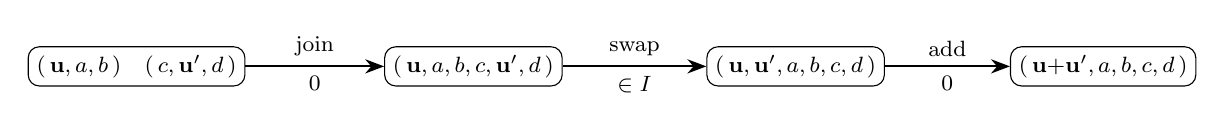
\begin{tikzpicture}[scale=0.93,every node/.style={font=\footnotesize}]
\node[draw,rounded corners,inner sep=3pt] (a) at (0,0) {$(\,\mathbf{u},a,b\,)\quad(\,c,\mathbf{u'},d\,)$};
\node[draw,rounded corners,inner sep=3pt] (b) at (4.6,0) {$(\,\mathbf{u},a,b,c,\mathbf{u'},d\,)$};
\node[draw,rounded corners,inner sep=3pt] (c) at (9.0,0) {$(\,\mathbf{u},\mathbf{u'},a,b,c,d\,)$};
\node[draw,rounded corners,inner sep=3pt] (d) at (13.2,0) {$(\,\mathbf{u}{+}\mathbf{u'},a,b,c,d\,)$};
\draw[vec] (a)--(b) node[midway,above] {join} node[midway,below] {$0$};
\draw[vec] (b)--(c) node[midway,above] {swap} node[midway,below] {$\in I$};
\draw[vec] (c)--(d) node[midway,above] {add} node[midway,below] {$0$};
\end{tikzpicture}
\caption{One merging step. Two closed sequences $(u,a,b)$ and $(c,u',d)$ contain a longest
entry $u$ and an equally long parallel entry $u'=tu$, $v(t)=0$. Join: they become the single sequence
$(u,a,b,c,u',d)$, and $S$ does not change. Swap: $u'$ is moved to the left past $c$, $b$, $a$; $S$
changes by $-2\det(a+b+c,u')$, a sum of three terms $2\det(\cdot,u')$ with valuation at least
$v(2)+\nu$. Add: $u,u'$ are replaced by $u+u'$, and $S$ does not change. The family has one entry
fewer.}\label{fig:merge}
\end{figure}

\begin{remark}\label{rem:M}
\begin{enumerate}[label=(\alph*)]
\item The factor $2$ comes only from Swap. The proof never divides by $2$, so Theorem~\ref{thm:M}
holds over any field and for any valuation (for instance also with $v(2)=0$, where it still gives a
correct, weaker statement).
\item Both choices in Step~1 are used: if $u$ is not a longest entry, Lemma~\ref{lem:T} is not
available in Step~2 (see the example after it); if $v(t)>0$, then $v(\det(u,w'))$ may drop below
$\nu$. In both cases flatness (not the inequality) can be lost; this happens in practice (control runs A and B in
Section~\ref{sec:comp}).
\item The proof is an algorithm: given the family and a way to compute $v$, it produces a sequence of
swaps whose costs add up to $S(F)$, each cost of valuation at least $v(2)+\nu$.
\end{enumerate}
\end{remark}

\begin{remark}[Theorem~\ref{thm:M} implies Rudenko's Theorem~1]\label{rem:rud}
Let $\Gamma$ be a finite trivalent graph with a $\Q^2$-valued flow $f$, as in \cite{Rud}: opposite
orientations of an edge carry opposite vectors, and the three vectors at a vertex sum to $0$. For
each vertex $x$ choose an order $e_1,e_2,e_3$ of the oriented edges with source $x$ and let
$c_x=(f(e_1),f(e_2),f(e_3))$. The family $F=(c_x)_x$ consists of closed sequences. It is balanced,
because its entries fall into pairs $f(e),-f(e)$. Put $\omega_x=\det(f(e_1),f(e_2))=\ar{c_x}$; the
determinant of any two different entries of $c_x$ is $\pm\omega_x$, so with $v=v_2$ the family is
$\nu$-flat for $\nu=\min_xv_2(\omega_x)$, which is Rudenko's weight $m(\Gamma,f)$.
Theorem~\ref{thm:M} gives $v_2\bigl(\sum_x\omega_x\bigr)\ge1+\nu$. If $\nu$ is finite, divide by
$2^\nu$: the terms with $v_2(\omega_x)=\nu$ become odd elements of $\Z_{(2)}$, the others even ones,
and the sum is even; so the number of vertices of minimal weight is even, which is \cite[Theorem
1]{Rud}. (If $\nu=\infty$, the statement is that the number of vertices of a trivalent graph is
even.) So Theorem~\ref{thm:M} contains Rudenko's graph theorem as the case $K=\Q$, $v=v_2$, sequences
of length three. The proofs are different: his is by a minimal counterexample and uses lattices
over $\Z_{(2)}$ and the residue field $\F_2$ \cite[Section 2]{Rud}; ours is the merging induction
above, which uses nothing about the valuation beyond (V1)--(V3). This comparison is ours and is not
Lean-verified.
\end{remark}

%=====================================================================
\section{Proof of the Key Proposition and of Stein's conjecture}\label{sec:end}

\begin{proof}[Proof of Proposition~\ref{thm:main}]
Let $t_1,\dots,t_n$ be the side sequences of the triangles, oriented counter-clockwise. Their
entries have coordinates in $K$, so $2\Area T_i=\ar{t_i}\in K$ and $2\Area P=\sum_i2\Area T_i\in K$.
The $t_i$ are closed; they form a $\nu$-flat family for $\nu=\min_iv(2\Area T_i)$ by \eqref{eq:tri};
the family is balanced by Lemma~\ref{lem:B}; and $S=2\Area P$. Apply Theorem~\ref{thm:M}.
\end{proof}

\begin{proof}[Proof of Corollary~\ref{cor:stein}]
Suppose all $T_i$ have area $a$ and $n=2m+1$. Let $K=\Q(\text{coordinates of the triangle
vertices})$, a countable field, and take $v$ on $K$ with $v(2)>0$ (Lemma~\ref{lem:V}). Then
$2\Area P=n\cdot2a$, and the Key Proposition gives $v(n)+v(2a)\ge v(2)+v(2a)$, so $v(n)>0$ (note
$a\ne0$). But $v(2m)\ge v(2)>0$, because $v\ge0$ on $\Z$ by (V3) (and $v(0)=\infty$), and $1=n-2m$,
so $0=v(1)\ge\min(v(n),v(2m))>0$, a contradiction.
\end{proof}

\begin{example}[the square cut by a diagonal, $v=v_2$]\label{ex:square}
The two triangles have the side sequences $t_1=((1,0),(0,1),(-1,-1))$ and
$t_2=((1,1),(-1,0),(0,-1))$; here $\nu=v_2(1)=0$ and $S=1+1=2$. All entries have $v=0$; take
$u=(1,0)$ and $u'=(-1,0)$, so $t=-1$. \emph{Join}:
$((1,0),(0,1),(-1,-1),(1,1),(-1,0),(0,-1))$, with bracket $2$. \emph{Swap}: moving $u'$ to the left
past the block $B=((0,1),(-1,-1),(1,1))$, whose sum is $(0,1)$, changes the bracket by
$-2\det(\sg(B),u')=-2\det((0,1),(-1,0))=-2$; the new sequence
$((1,0),(-1,0),(0,1),(-1,-1),(1,1),(0,-1))$ has bracket $0$. \emph{Add}: $u+u'=0$ is deleted; the
remaining sequence $((0,1),(-1,-1),(1,1),(0,-1))$ has bracket $0$, and the two further swaps change the
bracket by $+2$ and $-2$, nothing in total. So $S=2$ is exactly minus the total change made by the swaps, and the bound $v(S)\ge v(2)+\nu=1$
is attained. (Recomputed by the script \tL{run\_examples.py}.)
\end{example}

\begin{example}[the T-junction of Figure~\ref{fig:balance}, $v=v_2$]\label{ex:tj}
The side sequences are $B=((4,4),(-4,0),(0,-4))$, $A_1=((4,0),(-2,2),(-2,-2))$,
$A_2=((0,4),(-2,-2),(2,-2))$, with $2\Area=16,8,8$; so $\nu=3$, $S=32$, and the claim is
$v_2(S)\ge4$. The longest entries are the four with $v=1$. The procedure runs as follows (each line
gives the move and the change of $S$):
\begin{itemize}
\item $u=(-2,2)$ in $A_1$, $u'=(2,-2)$ in $A_2$: join $A_1A_2$; move $u'$ left past
$((-2,-2),(0,4),(-2,-2))$, change $-2\det((-4,0),(2,-2))=-16$; add, $u+u'=0$.
\item $u=u'=(-2,-2)$ in $((4,0),(-2,-2),(0,4),(-2,-2))$: move the second one left past $(0,4)$,
change $-2\det((0,4),(-2,-2))=-16$; add: $((4,0),(-4,-4),(0,4))$.
\item $u=(4,4)$ in $B$, $u'=(-4,-4)$: join; move $u'$ left past $((-4,0),(0,-4),(4,0))$, change
$-2\det((0,-4),(-4,-4))=+32$; add, $u+u'=0$; there remains $((-4,0),(0,-4),(4,0),(0,4))$.
\item $u=(-4,0)$, $u'=(4,0)$: change $-2\det((0,-4),(4,0))=-32$; add; then $(0,-4)$ and $(0,4)$
cancel at no cost.
\end{itemize}
The changes add up to $-32$, and the final family is empty, so $S=32$; each change is a multiple of
$16=2\cdot2^\nu$. The second step joins nothing and merges two \emph{equal} entries; the first and
third steps join different sequences. (Trace produced by \tL{run\_examples.py}.)
\end{example}

\begin{corollary}[a stronger form]\label{cor:strong}
Let a special polygon $P$ of area $A$ be dissected into triangles of areas $a_1,\dots,a_n$. Then
$\tfrac12$ belongs to the subring $\Z[a_1/A,\dots,a_n/A]$ of $\R$.
\end{corollary}

\begin{proof}
Let $K=\Q(\text{coordinates})$ and $R_0=\Z[a_1/A,\dots,a_n/A]\subseteq K$. If $\tfrac12\notin R_0$,
the construction in the proof of Lemma~\ref{lem:V}, started with $R_0$ instead of $\Z$, gives a
valuation ring $\cO\supseteq R_0$ of $K$ with $\tfrac12\notin\cO$, i.e.\ a valuation with
$v(a_i/A)\ge0$ for all $i$ and $v(2)>0$. Then $\min_iv(2a_i)\ge v(2A)$, and the Key Proposition gives
$v(2A)\ge v(2)+v(2A)$, so $v(2)\le0$, a contradiction.
\end{proof}

For the unit square ($A=1$) this says that $\tfrac12$ is an integer polynomial in the areas $a_i$;
this is the form in which Monsky states his theorem \cite[pp.~161--162]{Mon70}. For centrally
symmetric regions the corollary follows from \cite[Theorem 3.10]{Mon90} (for $A=2$, $1$ is an
integer polynomial without constant term in the $a_i$; divide by $2$). So the corollary is new at
most for special polygons that are not centrally symmetric.

%=====================================================================
\section{Complements}\label{sec:compl}

Nothing in this section is used in the proof of the Key Proposition, and nothing in it is formalised.

\subsection{Why a sum and not a count}

Let $v$ be a valuation with $v(2)>0$, let $\nu=\min_iv(2\Area T_i)$ and let $c=2\Area T_j$ for some
$j$ with $v(c)=\nu$. Dividing the Key Proposition by $c$ gives $v\bigl(\sum_i2\Area T_i/c\bigr)>0$;
the terms with $v(2\Area T_i)>\nu$ lie in $\m$, so
\[ \sum_{i:\ v(2\Area T_i)=\nu}\overline{2\Area T_i/c}=0\quad\text{in the residue field }k=\cO/\m. \]
For $k=\F_2$ every summand is $1$, and the statement says that the number of triangles of minimal
valuation is even; for $K=\Q$, $v=v_2$ this is the parity statement that Rudenko derives from his
Theorem~1. For larger $k$ the count can be odd.

\begin{example}\label{ex:fan}
Let $\phi=\frac{1+\sqrt5}2$ and $K=\Q(\sqrt5)$, with the valuation at the prime $2$, which is inert
in $K$; the residue field is $\F_4=\{0,1,\bar\phi,\bar\phi^2\}$. Cone the unit square from the point
$(\phi-1,\tfrac13)$. The four triangles have doubled areas $\tfrac13$ (bottom), $2-\phi$ (right),
$\tfrac23$ (top), $\phi-1$ (left). Since $\phi$ is a unit and $\phi-1=\phi^{-1}$,
$2-\phi=\phi^{-2}$, three of the four have valuation $0$: an odd number. Their residues relative to
$c=\tfrac13$ are $1$, $\bar\phi^{-2}=\bar\phi$ and $\bar\phi^{-1}=\bar\phi^2$ (using $3\equiv1$,
$\bar\phi^3=1$), and $1+\bar\phi+\bar\phi^2=0$ in $\F_4$, as the displayed formula requires.
(Recomputed exactly by \tL{run\_examples.py}.)
\end{example}

For an equidissection all residues are equal to $1$, so the vanishing sum again forces an even
count, whatever the residue field. So what the example shows is this: when the residue field is
larger than $\F_2$, the number of triangles of minimal valuation need not be even, while the
weighted sum of residues still vanishes. It does not show that no parity argument can be made to
work over such fields.

\subsection{``Special'' is sufficient, not necessary}\label{sec:trap}

The converse of Stein's conjecture fails: there are non-special polygons without odd
equidissections. Consider a trapezoid whose parallel sides have ratio $p/q$, with $p\ne q$ coprime
positive integers. It is the image under an affine map of the trapezoid $Z$ with vertices
$(0,0),(q,0),(p,1),(0,1)$, of area $\frac{p+q}2$.

\begin{proposition}[known; see below]\label{prop:trap}
The trapezoid $Z$ has an odd equidissection if and only if $p+q$ is odd.
\end{proposition}

The set of all $n$ for which the trapezoid with ratio $r/s$ (in lowest
terms) has an equidissection into $n$ triangles is the set of multiples of $r+s$: this is
\cite[Theorem 3.2]{KS} (Kasimatis and Stein) and \cite[Chapter 5, Theorem 3, pp.~122--123]{SS}.
Proposition~\ref{prop:trap} is a special case of this. The proof there is in substance the one
below, applied to every prime $p$ dividing $r+s$: Monsky's colouring for a valuation of $\R$
extending the $p$-adic one, Sperner's lemma, and the bound for the area of a triangle with three
colours (\cite[Theorem 0.1]{KS}, \cite[Chapter 5, Lemmas 1--3]{SS}). Both sources give the argument
for simplicial dissections; \cite[p.~107]{SS} adds that ``the theorems hold for all dissections''.
The proof below is by Monsky's colouring method. The
colouring and the properties of Lemma~\ref{lem:col} are in \cite[p.~163]{Mon70} for an ultranorm
on $\R$ with $\|2\|<1$, and in \cite[Section 2, Lemma
1]{Rud12}, attributed there to Monsky \cite{Mon70}, for a valuation of $\R$ extending $v_2$ (with
the bound $-1$ in place of $-v(2)$; his colours $A,B,C$ are our $1,3,2$); \cite[p.~158]{AZ} has
them for a valuation with values in an ordered group. We prove the two lemmas we
need for an arbitrary valuation with $v(2)>0$ on the coordinate field, and claim no novelty for
them.

Let $v$ be a valuation on a field $K\subset\R$ with $v(2)>0$. Colour a point $(x,y)\in K^2$ with
colour $1$ if $v(x)>0$ and $v(y)>0$; with colour $2$ if it has not colour $1$ and $v(x)\le v(y)$
(then $v(x)\le0$); with colour $3$ otherwise (then $v(y)\le0$ and $v(y)<v(x)$).

\begin{lemma}[Monsky's colouring, for a general valuation]\label{lem:col}
\begin{enumerate}[label=(\alph*)]
\item If $z\in K^2$ has colour $1$, then $w$ and $w-z$ have the same colour, for every $w\in K^2$.
\item If $z_1,z_2,z_3$ have colours $1,2,3$, then $v(\det(z_2-z_1,z_3-z_1))\le0$. In particular they
are not collinear, so a line contains points of at most two colours; and the triangle
$z_1z_2z_3$ has an area of valuation at most $-v(2)<0$.
\end{enumerate}
\end{lemma}

\begin{proof}
(a) Let $z=(a,b)$ with $v(a),v(b)>0$ and $w=(x,y)$. If $w$ has colour $1$, so has $w-z$ by (V3). If
$w$ has colour $2$, then $v(x)\le0<v(a)$, so $v(x-a)=v(x)$, and
$v(y-b)\ge\min(v(y),v(b))\ge v(x)$; so $w-z$ has colour $2$. If $w$ has colour $3$, then
$v(y-b)=v(y)\le0$ and $v(x-a)\ge\min(v(x),v(a))>v(y)$; so $w-z$ has colour $3$. (We used that
$v(s+t)=v(s)$ if $v(s)<v(t)$, a consequence of (V3).)
(b) By (a) we may subtract $z_1$ and assume $z_1=0$. With $z_2=(x_2,y_2)$ of colour $2$ and
$z_3=(x_3,y_3)$ of colour $3$, we have $v(x_2y_3)=v(x_2)+v(y_3)\le0$ and
$v(x_3y_2)=v(x_3)+v(y_2)>v(y_3)+v(x_2)$. Hence $v(\det(z_2,z_3))=v(x_2y_3-x_3y_2)=v(x_2)+v(y_3)\le0$.
The area is $\tfrac12|\det|$.
\end{proof}

\begin{lemma}[Sperner-type count, with T-junctions]\label{lem:sperner}
Let a polygon $P$ be dissected into triangles with vertices in $K^2$, and let the vertices of $P$ be
in $K^2$. Cut the sides of the triangles and the edges of $P$ into pieces as in the proof of
Lemma~\ref{lem:B}, and call a piece a \emph{$12$-piece} if its end points have colours $1$ and $2$.
If the number of $12$-pieces on $\partial P$ is odd, then some triangle of the dissection has
vertices of three different colours.
\end{lemma}

\begin{proof}
First, let $s$ be a segment whose end points are nodes, cut into pieces at the nodes on it. By
Lemma~\ref{lem:col}(b) the nodes on $s$ have at most two colours. If colour $3$ occurs among them,
$s$ contains no $12$-piece. Otherwise all nodes on $s$ have colours $1$ or $2$, and the number of
$12$-pieces on $s$ is odd if and only if the end points of $s$ have different colours. In both cases
the number of $12$-pieces on $s$ is odd if and only if the end points of $s$ have colours $1$ and
$2$. Next, a triangle has an odd number of sides with end points of colours $1$ and $2$ if and only
if its vertices have three different colours (check the cases: colours $\{1,2,3\}$ give one such
side; colours within $\{1,2\}$ give none or two; all other cases give none). So the number $N_T$ of
$12$-pieces on the three sides of a triangle $T$ is odd exactly for the triangles with three
colours. Finally, by the proof of Lemma~\ref{lem:B}, a piece inside $P$ lies on exactly two triangle
sides and a piece on $\partial P$ on exactly one. Hence $\sum_TN_T$ is twice the number of
$12$-pieces inside $P$ plus the number of $12$-pieces on $\partial P$, and the claim follows.
\end{proof}

\begin{proof}[Proof of Proposition~\ref{prop:trap}]
If $p+q$ is odd, triangulate $Z$ using the integer points on the two bases: the $q$ unit segments of
the lower base and the $p$ unit segments of the upper base are the bases of $p+q$ triangles of area
$\tfrac12$ that fill the strip.

Let $p+q$ be even; then $p$ and $q$ are both odd, being coprime. Suppose there is an equidissection
into an odd number $n$ of triangles. Let $K=\Q(\text{coordinates})$ and take $v$ on $K$ with $v(2)>0$
(Lemma~\ref{lem:V}). Odd integers have valuation $0$ (if $v(k)>0$ for $k=2j+1$, then
$v(1)\ge\min(v(k),v(2j))>0$). Each triangle has area $\frac{p+q}{2n}$, of valuation
$v(p+q)-v(2)-v(n)\ge0$, since $p+q$ is even and $n$ is odd. By Lemma~\ref{lem:col}(b) no triangle
has vertices of three colours, so by Lemma~\ref{lem:sperner} the number of $12$-pieces on
$\partial Z$ is even. But the corners $(0,0),(q,0),(p,1),(0,1)$ have colours $1,2,2,3$. On the lower
base ($y=0$) only the colours $1$ and $2$ occur, and it goes from colour $1$ to colour $2$, so it
contains an odd number of $12$-pieces. The right side has both ends of colour $2$, so it contains an
even number (first part of the proof of Lemma~\ref{lem:sperner}). The upper base ($y=1$) has no point
of colour $1$, and the left side ($x=0$) no point of colour $2$. The total is odd, a contradiction.
\end{proof}

%=====================================================================
\section{Which special polygons do the methods cover?}\label{sec:scope}

The problem statement asks for clarity on this point. Table~\ref{tab:coverage} records what is
known, with the statements and methods on which each row rests.

\begin{table}[!htbp]
\centering\small
\begin{tabular}{@{}>{\raggedright\arraybackslash}p{3.3cm}>{\raggedright\arraybackslash}p{3.7cm}>{\raggedright\arraybackslash}p{2.6cm}>{\raggedright\arraybackslash}p{5.2cm}@{}}
\toprule
Source & Polygons & Coordinates of the triangle vertices & Statement and method\\
\midrule
Monsky \cite{Mon70} & square (hence parallelograms, by an affine map) & real & \cite[pp.~161--164]{Mon70}. Colouring of the plane in three sets by an extension of the $2$-adic absolute value to $\R$, and a lemma of Sperner type.\\
Monsky \cite{Mon90} & centrally symmetric regions: any $S=-S$ that is a finite union of non-overlapping triangles & real & \cite[Theorems 3.8, 3.10]{Mon90}. Tricolourings and a homological argument in a group of closed chains of segments; an ``almost discrete'' valuation ring with $2$ in its maximal ideal.\\
Stein \cite{Ste00} & special polygons with at most six sides & real & \cite[Theorems 1, 2]{Ste00}. Monsky's colouring for a $2$-adic valuation on $\R$, after affine maps chosen case by case.\\
Stein \cite{Ste99}, Praton \cite{Pra} & polyominoes: an odd number of squares \cite{Ste99}; all \cite{Pra} & not restricted in the statements; the labelling is written for rational points & \cite[p.~256]{Ste99}, \cite[Theorem 6]{Pra}. Monsky's colouring after maps $(x,y)\mapsto(x/2^r,y/2^s)$, and a count of labelled boundary edges \cite[Chapter 5]{SS}.\\
Rudenko \cite{Rud12} & balanced polygons with integer vertices and odd area & real (as far as we know) & Monsky's colouring and a homology class of the boundary.\\
Rudenko \cite{Rud} & all special polygons & rational & \cite[Theorems 1, 2]{Rud}. Flows on trivalent graphs, lattices over $\Z_{(2)}$.\\
This report & all special polygons & real & Proposition~\ref{thm:main}, Corollary~\ref{cor:stein}: not peer-reviewed; Lean-verified as in Section~\ref{sec:lean}.\\
\bottomrule
\end{tabular}
\caption{Coverage of the methods.}\label{tab:coverage}
\end{table}

Four remarks. A corner of $P$ (a vertex at which the boundary turns) is a vertex of some
triangle of every dissection (near a corner, a triangle that does not have it as a vertex is a
half-disc, and half-discs alone cannot fill an angle different from $\pi$; this is elementary and
not formalised), so a polygon that has a dissection with rational vertices has rational
corners: the row of \cite{Rud} concerns special polygons with rational corners only, and among
their dissections only the rational ones. Next, in the rows above ours the gap is the combination ``all special polygons'' and
``irrational coordinates'': for example a polygon with eight sides parallel to the axes that is
neither centrally symmetric nor an affine image of a polyomino (its horizontal side lengths are
not rational multiples of one another), dissected arbitrarily. L-shaped hexagons are covered by
\cite[Theorem 1]{Ste00}; Stein's remark on ``several families'' with more than six sides
\cite[p.~145]{Ste00} names no family. For a polyomino dissected with irrational vertices, the
statements of \cite{Ste99,Pra} carry no restriction, but the two papers define the labelling for
rational points only.
Third, our method needs nothing about $P$ beyond the balance lemma, so it applies verbatim to any
region for which the conclusion of Lemma~\ref{lem:B} holds with vanishing right-hand side. Fourth,
the method gives divisibility by $2$ and nothing more, and by Proposition~\ref{prop:trap} the class
of special polygons is not the exact class of polygons without odd equidissections.

%=====================================================================
\section{Formalisation in Lean}\label{sec:lean}

A Lean~4 project (library \tL{Stein}; Lean v4.35.0, Mathlib v4.35.0, no other dependency;
about 6\,500 lines) accompanies this report. Its file \tL{README.md} gives the full correspondence;
this section states what the report relies on.

\textbf{Check.} The project builds (``Build completed successfully''); its source contains no
\tL{sorry} and no \tL{native\_decide}; and for each declaration named in Table~\ref{tab:lean},
\tL{\#print axioms} reports a subset of \tL{propext}, \tL{Classical.choice}, \tL{Quot.sound}. This
is recorded in the file \tL{lean-check-output.txt} of the project. In
this report, \emph{Lean-verified} is used only for these declarations.

\textbf{The formal statements, in words.} Points are elements of $\R\times\R$.
\begin{itemize}
\item \tL{SimplePolygon P}, for $P\colon\{0,\dots,m+2\}\to\R^2$ (at least three vertices): the
vertices are pairwise distinct, and two different sides $[P_k,P_{k+1}]$ (indices cyclic) have a
common point only if they are consecutive, and then only the common vertex. Collinear consecutive
sides are allowed.
\item \tL{region P}: the union of the sides and of the set of points with non-zero winding number,
where the winding number is defined as the sum of the signed angles under which the sides are seen
from the point, divided by $2\pi$ and rounded. This is the polygon $P$ of Section~\ref{sec:intro}.
That it is the usual closed region bounded by the curve is itself Lean-verified, see the row
``the region'' of Table~\ref{tab:lean}.
\item \tL{SpecialPolygon P}: for every $d\ne0$, the sum of those vectors $P_{k+1}-P_k$ that are
parallel to $d$ is $0$ (Definition~\ref{def:special}; no orientation is assumed).
\item \tL{IsTriangle T}: $T$ is the convex hull of three non-collinear points. \tL{IsTriangleOver K
T}: the same with the three points in $K^2$, for a subfield $K$ of $\R$.
\item \tL{IsDissection S T}: every $T_i$ is a triangle, the interiors of $T_i$ and $T_j$ are
disjoint for $i\ne j$, and $\bigcup_iT_i=S$. T-junctions are allowed.
\item Areas are \tL{MeasureTheory.volume}, i.e.\ Lebesgue measure on $\R^2$.
\item Valuations are Mathlib's \tL{Valuation K $\Gamma_0$}, written multiplicatively: $|x|=$
``$\exp(-v(x))$'' with values in a linearly ordered commutative group with zero. So $v(x)\ge\nu$
reads $|x|\le\gamma$, the condition $v(2)>0$ reads $|2|<1$, and the Key Proposition reads: \emph{if
$|a_i|\le\gamma$ for all $i$, then $|a_0|\le|2|\cdot\gamma$}, where $a_i,a_0\in K$ are given
together with the hypotheses that their real values are $2\Area T_i$ and $2\Area P$. Using an upper
bound $\gamma$ in place of the minimum is equivalent.
\end{itemize}

The two headline statements, copied from the file \tL{Stein/Main.lean} (Unicode
symbols transliterated: \tL{R} for the reals, \tL{->} for the arrow, \tL{forall}, \tL{<=}, \tL{I}
for the index type $\iota$, \tL{G0} for $\Gamma_0$, \tL{a0} for $a_0$, \tL{g} for $\gamma$):
{\footnotesize
\begin{verbatim}
theorem stein_conjecture (P : Fin (m + 3) -> R x R) (hP : SimplePolygon P) (hsp : SpecialPolygon P)
    {I : Type*} [Fintype I] (T : I -> Set (R x R)) (hT : IsDissection (region P) T)
    (heq : forall i j, volume (T i) = volume (T j)) : Even (Fintype.card I)

theorem main_theorem (P : Fin (m + 3) -> R x R) (hP : SimplePolygon P) (hsp : SpecialPolygon P)
    {I : Type*} [Fintype I] (T : I -> Set (R x R)) (hT : IsDissection (region P) T)
    (K : Subfield R) (hK : forall i, IsTriangleOver K (T i))
    {G0 : Type*} [LinearOrderedCommGroupWithZero G0] (v : Valuation K G0) (g : G0)
    (a : I -> K) (ha : forall i, (a i : R) = 2 * (volume (T i)).toReal)
    (hg : forall i, v (a i) <= g)
    (a0 : K) (ha0 : (a0 : R) = 2 * (volume (region P)).toReal) :
    v a0 <= v 2 * g
\end{verbatim}}

{\small
\begin{longtable}{@{}>{\raggedright\arraybackslash}p{3.5cm}>{\raggedright\arraybackslash}p{4.6cm}>{\raggedright\arraybackslash}p{6.6cm}@{}}
\caption{Claims of the report and the Lean declarations that support them. All declarations in the
second column are Lean-verified in the sense above.}\label{tab:lean}\\
\toprule
Claim & Lean declaration & Differences between the formal statement (or proof) and the text\\
\midrule
\endfirsthead
\toprule
Claim & Lean declaration & Differences\\
\midrule
\endhead
\bottomrule
\endfoot
Lemma~\ref{lem:V} & \tL{Stein.exists\_valuation\_\allowbreak two\_pos} & Statement: \emph{every} field of characteristic $0$ has a valuation ring with $|2|<1$. Proof: from Mathlib's existence theorem for valuation subrings, which uses Zorn's lemma. \textbf{The construction for countable fields in Appendix~\ref{sec:proofV} (the Claim and the iteration) is not formalised.}\\
Formula \eqref{eq:C}; Lemma~\ref{lem:moves} (a), (b), (c) & \tL{Stein.bracket\_append}, \tL{bracket\_join}, \tL{bracket\_swap}, \tL{bracket\_add} & None; any commutative ring; signs as in Lemma~\ref{lem:moves}.\\
Formula \eqref{eq:tri} & \tL{Stein.bracket\_sideSeq}, \tL{det\_sideSeq} & \tL{det\_sideSeq} allows a third case $\det(w,w')=0$ (for $w=w'$).\\
Lemma~\ref{lem:T} & \tL{Stein.lemma\_T} & None.\\
Theorem~\ref{thm:M} & \tL{Stein.theorem\_M} & None: any field, any valuation; in Lean a family is a \tL{List} of \tL{List}s; $\nu=\infty$ allowed. The formal proof follows Steps 1--4 of the text.\\
Proposition~\ref{fact:P} (P1), (P2) & \tL{Stein.Polygon.\allowbreak frontier\_region}, \tL{Stein.Polygon.\allowbreak region\_orientedBoundary} & (P2) is stated as: \tL{region P} lies on the left of all sides $P_k\to P_{k+1}$, or on the left of all reversed sides. Which case holds is decided by the sign of the shoelace sum (\tL{region\_orientedBoundary\_\allowbreak of\_shoelace\_pos}).\\
The region: \tL{region P} is the usual closed region bounded by a simple closed polygon (used in the text only to justify the definition of $P$) & \tL{Stein.Polygon.jordan}, \tL{closure\_inner}, \tL{region\_eq\_bounded}, \tL{region\_eq\_polyInterior}, \tL{mem\_region\_iff\_\allowbreak odd\_crossings}, \tL{volume\_region}, \tL{shoelace\_pos\_iff}, \tL{region\_eq\_convexHull}, \tL{region\_unitSquare} (all in \tL{Stein.Polygon}) & \tL{jordan}: the complement of the curve is the disjoint union of \tL{region P} minus the curve and the complement of \tL{region P}; both are open and connected, the first is bounded, the second is not. \tL{closure\_inner}, \tL{region\_eq\_bounded}, \tL{region\_eq\_polyInterior}: \tL{region P} is the closure of the first set, and equals the curve together with the points whose component in the complement of the curve is bounded. \tL{mem\_region\_iff\_odd\_crossings}: ray-crossing parity, \emph{only for rays through no vertex}. \tL{volume\_region}: the area is $\tfrac12|\text{shoelace sum}|$; \tL{shoelace\_pos\_iff}: the sum is positive if and only if the winding number takes only the values $0$ and $1$ off the curve (counter-clockwise order). \tL{region\_eq\_convexHull}: for a \emph{strictly} convex counter-clockwise polygon the region is the convex hull; \tL{region\_unitSquare}: for the unit square it is $[0,1]^2$. ``Exactly two components'' is expressed through the components of points, not as a statement about the number of components.\\
Lemma~\ref{lem:B} (Balance) & \tL{Stein.balance}, \tL{Stein.balanced\_\allowbreak of\_special} & Statement: as in the text, for any set $S$ with a finite list of oriented sides such that (i) a point on no side has a neighbourhood inside $S$ or a neighbourhood outside $S$, (ii) the half-disc property (P2) holds at every point that lies on exactly one side and is not an end point of it, (iii) two different sides have finitely many common points (\tL{Stein.OrientedBoundary}; this includes regions with holes). \textbf{The formal proof is not the proof of Section~\ref{sec:balance}}: it compares, across a line, the jumps of the indicator functions of the triangles and of the region, and integrates along the line. The cutting into pieces is not formalised.\\
Area of a triangle; additivity of area & \tL{Stein.volume\_triangle}, \tL{Stein.IsDissection.\allowbreak volume\_eq\_sum} & None (Lebesgue measure).\\
Proposition~\ref{thm:main} & \tL{Stein.main\_theorem}; also \tL{main\_theorem\_\allowbreak of\_orientedBoundary}, \tL{main\_theorem\_square} & Multiplicative notation and the elements $a_i,a_0$, as explained above; that $2\Area T_i$ and $2\Area P$ lie in $K$ is thus a hypothesis of the formal statement, while in Proposition~\ref{thm:main} it is a conclusion (proved in the text in one line). $K$ is a subfield of $\R$ containing the coordinates of the triangle vertices. The polygon is a vertex list with \tL{SimplePolygon}.\\
Corollary~\ref{cor:stein} (Stein) & \tL{Stein.stein\_conjecture}, \tL{Stein.stein\_conjecture\_fin}; also \tL{stein\_conjecture\_\allowbreak of\_orientedBoundary} & Conclusion: the number of triangles is even. Proved with $K=\R$ and Lemma~\ref{lem:V} for $\R$ (hence with Zorn's lemma), not with $K=\Q(\text{coordinates})$.\\
Corollary~\ref{cor:stein} (Monsky) & \tL{Stein.monsky}, \tL{Stein.monsky\_fin} & The square is $[0,1]^2$; proved directly, without the general polygon part (\tL{Stein.square\_boundary}).\\
\end{longtable}}

\textbf{The official statement.} The organisers' Lean statement of the problem, \tL{Mathathon.P67.Monsky} (for $n\in\mathbb N$: the unit square, as a subset of \tL{EuclideanSpace R (Fin 2)}, is the union of a finite set of $n$ triangles with pairwise disjoint open hulls and equal areas if and only if $n\ne0$ and $n$ is even), is proved in a second file, \tL{MathathonProblems/P67\_Monsky.lean}, with the statement and its definitions unchanged and only the proof added. The direction ``$\Rightarrow$'' is \tL{Stein.monsky} after a measure-preserving change of coordinates; the direction ``$\Leftarrow$'' is an explicit dissection into $n/2$ vertical strips, each cut by a diagonal. \tL{\#print axioms} for \tL{Mathathon.P67.Monsky} reports \tL{propext}, \tL{Classical.choice}, \tL{Quot.sound}.

\textbf{Not formalised.} The countable construction in Lemma~\ref{lem:V}; the hand proof of
Lemma~\ref{lem:B}; ray-crossing parity for rays through a vertex; the identification of the region
with the convex hull for convex polygons that are clockwise or not strictly convex; Lemma~\ref{lem:examples}; the examples; Remark~\ref{rem:rud};
Corollary~\ref{cor:strong}; all of Section~\ref{sec:compl}.

\textbf{What the formalisation does and does not show.} It shows that the statement \tL{Stein.stein\_conjecture}
follows from the axioms of Lean and Mathlib: for a simple closed polygon given by its vertices, with
the region defined by the winding number (and proved to be the closure of the bounded component of
the complement of the curve), and with Lebesgue areas, a special polygon has no odd
equidissection. The reader should check that the definitions above say what is intended; this is
the one place where a formal proof can differ from the claim. It does not show that the proof
avoids the axiom of choice (\tL{Classical.choice} is used throughout Mathlib): the statement that
Lemma~\ref{lem:V} needs no Zorn's lemma for countable fields is a claim about the hand proof in
Appendix~\ref{sec:proofV}. And it is not a judgement on novelty.

%=====================================================================
\section{Checks by computation}\label{sec:comp}

The proof of Theorem~\ref{thm:M} is an algorithm (Remark~\ref{rem:M}(c)). We implemented it in
Python with exact arithmetic (\tL{fractions.Fraction}, and an exact class for $\Q(\sqrt d)$); no
floating-point numbers are used. The scripts and their logs are in the folder \tL{code} of the
repository: \tL{merge.py} (fields, valuations, brackets, the procedure), \tL{dissect.py} (polygons
and random dissections), \tL{run\_examples.py}, \tL{run\_random.py}, \tL{run\_controls.py}, and
\tL{logs/}. The computations test the mechanism of the proof on examples. They cannot test
Corollary~\ref{cor:stein} directly, since there are no odd equidissections to generate, and they
prove nothing.

\textbf{What the procedure asserts.} After every move: all sequences are closed; the family is
$\nu$-flat (all pairs of entries of the modified sequence); the family is balanced; a join and an
add leave $S$ unchanged; a swap of neighbours $p,q$ changes the bracket by exactly $-2\det(p,q)$ and
this has valuation $\ge v(2)+\nu$; in Step~1 a partner with $v(t)=0$ exists. At the end: the swap
costs add up to $S$, and $v(S)\ge v(2)+\nu$.

\textbf{Valuations used.} $v_2,v_3,v_5$ on $\Q$; the valuation of $\Q(\sqrt5)$ at the inert prime
$2$ (residue field $\F_4$); the valuation of $\Q(\sqrt2)$ at the ramified prime $\sqrt2$, normalised
with $v(\sqrt2)=1$, $v(2)=2$. For the last two, (V2) and (V3) were tested on 4998 and 5000 random pairs.

\textbf{Dissections.} A random special polygon is one of: the unit square; a parallelogram; a
centrally symmetric convex hexagon or octagon (sums of random segments); one of seven polyominoes
with three to five cells, or its image under a random affine map; all with random coordinates in
the field. It is triangulated in a fixed way and then refined by 2 to 12 random steps (2 to 9 over
the quadratic fields), each of which subdivides \emph{one} triangle: by a new vertex inside it, or
by a new vertex on one of its sides, or by new vertices on two of its sides. The last two kinds
create T-junctions with the neighbouring triangles. For every instance the script also checks the
conclusion of Lemma~\ref{lem:B} directly (for every direction, the triangle side vectors and the
edge vectors of the polygon have the same sum).

\textbf{Results} (logs \tL{examples.log}, \tL{random.log}, \tL{controls.log}; seeds are recorded in
the logs).
\begin{enumerate}
\item \emph{Worked examples} (\tL{run\_examples.py}): the numbers of the example after
Lemma~\ref{lem:T} and of Examples~\ref{ex:square}, \ref{ex:tj} and \ref{ex:fan}, and the trapezoid
of Section~\ref{sec:intro}, were recomputed and agree with the text.
\item \emph{Random dissections of special polygons} (\tL{run\_random.py}): 4800 dissections with
73\,064 triangles in total (at most 31 per dissection), of which 4589 contain at least one
T-junction: 2000 over $\Q$ with $v_2$, 1000 each over $\Q$ with $v_3$ and $v_5$, 400 over
$\Q(\sqrt5)$ and 400 over $\Q(\sqrt2)$ with the valuations above. The procedure made 65\,877 joins,
414\,440 swaps and 130\,743 adds. \emph{No assertion failed.} In particular the balance lemma and
the inequality of the Key Proposition held in all 4800 instances. The bound was attained, i.e.\
$v(S)=v(2)+\nu$, in 102 of the 2000 instances with $v_2$.
\item \emph{Sum against count.} Over $\Q$ with $v_2$ the number of triangles of minimal valuation was
even in all 2000 instances. Over $\Q(\sqrt5)$ the sum of the residues in $\F_4$ vanished in all 400
instances, and the number of triangles of minimal valuation was odd in 7 of them. In a further
4000 instances of the type of Example~\ref{ex:fan} (the unit square coned from a random point with
coordinates in $\Q(\sqrt5)$), the residue sum vanished in all, and the count was odd in 40.
\item \emph{Other primes.} For $v_3$ and $v_5$ Theorem~\ref{thm:M} holds (with $v(2)=0$) and all
assertions passed; but the analogous inequality with $v(p)$ in place of $v(2)$ failed in 212 of
1000 instances for $p=3$ and in 318 of 1000 for $p=5$. The gain is specific to the factor $2$ of
the swap.
\item \emph{Controls, one hypothesis removed at a time} (\tL{run\_controls.py}; 1000 instances over
$\Q$ with $v_2$ and 250 over $\Q(\sqrt5)$ for each of A, B, C).
\begin{itemize}
\item[A.] \emph{$u$ not a longest entry} (chosen among the entries of non-minimal valuation that
have a partner with $v(t)=0$): flatness was lost in a join in 617 of 1000 instances over $\Q$ and
in 156 of 250 over $\Q(\sqrt5)$; the other runs completed.
\item[B.] \emph{Partner with $v(t)>0$} (whenever the longest entry has one): flatness was lost in a
join in 334 of 1000 and in 84 of 250 instances; the other runs completed (in 6 instances no such
partner ever existed).
\item[C.] \emph{Polygon not special} (trapezoids, triangles, convex quadrilaterals, refined in the
same way): the family is not balanced, and in all 1250 instances the procedure stopped in Step~1
because no partner existed. The inequality $v(S)\ge v(2)+\nu$ itself failed in 87 of 1000 instances
over $\Q$ and in 13 of 250 over $\Q(\sqrt5)$.
\item[D.] \emph{Lemma~\ref{lem:T} without ``$u$ at least as long as $w,w'$''}: among 19\,947 random
triples over $\Q$ with $v_2$, the conclusion held in all 8940 triples satisfying the hypothesis, and
failed in 4729 of the 11\,007 triples violating it.
\end{itemize}
In controls A and B the final inequality cannot fail (it is a theorem); what fails is the invariant
on which the proof relies, which shows that both choices in Step~1 are needed for this proof.
\end{enumerate}

%=====================================================================
\section{Work done during the event}\label{sec:event}

Before the event we only familiarised ourselves with the problem statement. All of the work
listed below was done during the 40 hours of the event.

The submission contains the following work that is not taken from the literature.
\begin{enumerate}
\item The statement and proof of Theorem~\ref{thm:M} (merging induction; for its relation to
\cite{Rud12} see Section~\ref{sec:known}) and of the Key Proposition for
an arbitrary valuation, with Lemma~\ref{lem:T}; the deduction of Stein's conjecture for real
coordinates and of Corollary~\ref{cor:strong}.
\item A complete write-up of the balance lemma with T-junctions (Lemma~\ref{lem:B}), and the
iterated form of the existence lemma for countable fields (Lemma~\ref{lem:V}).
\item The comparison with Rudenko's theorem (Remark~\ref{rem:rud}); the residue-field formula and
the example over $\Q(\sqrt5)$; the proof of the trapezoid proposition for a general valuation
(Section~\ref{sec:compl}).
\item The Lean project of Section~\ref{sec:lean}, including a formal proof of the Jordan curve theorem for
simple closed polygons and of the facts about simple polygons that the balance lemma needs. Its build log and check output are dated 14--15 November
2026 (UTC).
\item The exact-arithmetic implementation and the runs of Section~\ref{sec:comp} (logs dated
14 November 2026).
\item The literature check described in Section~\ref{sec:limits}, item~2.
\end{enumerate}
Not event work: the results quoted in Section~\ref{sec:known}. Lemma~\ref{lem:V} (a key step of the
classical existence proof for valuation rings), Lemma~\ref{lem:B} (additivity under dissection),
the identities of Lemma~\ref{lem:moves}, Lemma~\ref{lem:col} (Monsky's colouring) and
Proposition~\ref{prop:trap} are classical, elementary or known; the work in them is the
presentation.

%=====================================================================
\section{How each main claim is supported}\label{sec:support}

Table~\ref{tab:support} is the single record of the status of every claim. ``Proved here'' means
that a complete proof is in this report. ``Lean-verified'' refers to Table~\ref{tab:lean} and has
the meaning fixed in Section~\ref{sec:lean}. ``Computed'' refers to Section~\ref{sec:comp} and means
tested on the stated instances, not proved. No entry has been peer-reviewed.

{\small
\begin{longtable}{@{}>{\raggedright\arraybackslash}p{5.2cm}>{\raggedright\arraybackslash}p{9.8cm}@{}}
\caption{Support for each claim.}\label{tab:support}\\
\toprule
Claim & Support\\
\midrule
\endfirsthead
\toprule
Claim & Support\\
\midrule
\endhead
\bottomrule
\endfoot
Lemma~\ref{lem:examples} (examples of special polygons) & Proved here.\\
Lemma~\ref{lem:V} (valuation with $v(2)>0$) & Proved here for countable fields, without Zorn's lemma. Lean-verified for all fields of characteristic $0$, by a different (Zorn-based) proof. Classical.\\
Lemma~\ref{lem:moves}, formulas \eqref{eq:C}, \eqref{eq:tri} & Proved here. Lean-verified. Computed (every move of every run).\\
Proposition~\ref{fact:P} (local structure of a simple polygon); the Jordan curve theorem for simple closed polygons and the equivalent descriptions of $P$ & Lean-verified. Not proved here.\\
Area of a triangle, additivity of area & Standard measure theory; one-line argument in Section~\ref{sec:seq}. Lean-verified.\\
Lemma~\ref{lem:B} (balance) & Proved here from Proposition~\ref{fact:P}. Statement Lean-verified, by a different proof. Computed on all random instances.\\
Lemma~\ref{lem:T} & Proved here. Lean-verified. Computed (control D).\\
Theorem~\ref{thm:M} & Proved here. Lean-verified (same proof). Computed on all random instances.\\
Proposition~\ref{thm:main} (Key Proposition) & \textbf{Not peer-reviewed.} Proved here from the items above. Lean-verified in the form of Section~\ref{sec:lean}. Computed on all random instances.\\
Corollary~\ref{cor:stein} (Stein's conjecture for real coordinates; Monsky's theorem) & \textbf{Not peer-reviewed.} Proved here from Proposition~\ref{thm:main} and Lemma~\ref{lem:V}. Lean-verified in the form of Section~\ref{sec:lean}. Monsky's theorem itself is known \cite{Mon70}.\\
Corollary~\ref{cor:strong} (stronger form) & Proved here from Proposition~\ref{thm:main} and the proof of Lemma~\ref{lem:V}. Known for the square \cite{Mon70} and for centrally symmetric regions \cite{Mon90}. Not formalised.\\
Remark~\ref{rem:rud} (Theorem~\ref{thm:M} implies Rudenko's Theorem~1) & Proved here. Not formalised.\\
Residue-field formula, Example~\ref{ex:fan}; Examples~\ref{ex:square}, \ref{ex:tj} & Proved here; the numbers computed exactly. Not formalised.\\
Lemmas~\ref{lem:col}, \ref{lem:sperner}, Proposition~\ref{prop:trap} (trapezoids) & Proved here. The proposition is known (\cite[Theorem 3.2]{KS}, \cite[p.~122]{SS}; proved there by the same method); the colouring lemma is Monsky's \cite[p.~163]{Mon70}. Not formalised.\\
Known results of Section~\ref{sec:known}, Table~\ref{tab:coverage} & Cited.\\
``The real case was not known before'' & To the best of our knowledge this has not been shown before. See Section~\ref{sec:limits}.\\
\end{longtable}}

%=====================================================================
\section{Limitations, novelty and next steps}\label{sec:limits}

\begin{enumerate}
\item \textbf{Not peer-reviewed.} The team checked the whole proof, and the deductions are
Lean-verified, but no outside expert has been consulted. Lean does not replace an expert's
judgement of the definitions or of the relation to the literature.
\item \textbf{Novelty.} We searched arXiv (all versions up to November 2026), zbMATH Open,
OpenAlex (including papers citing Monsky, Stein and Praton), Semantic Scholar, MathOverflow and
Math StackExchange, and the general web, including Russian, Chinese, German and French sources.
For some papers found this way only the zbMATH reviews were read. Google Scholar and MathSciNet
were not queried, the papers citing \cite{Rud} could not be retrieved, and Stein's survey in the
\emph{Mathematical Intelligencer} 26 (2004), 17--21, was not read. None of the sources found proves
the conjecture for special polygons with real coordinates, and none contains a merging argument. To
the best of our knowledge the result is new.
\item \textbf{The definition of ``special''} is Stein's \cite[p.~141]{Ste00}. The balanced polygons
of \cite{Rud12} (edges in pairs of parallel, equally long, opposite edges) are special, and a special
polygon becomes balanced after subdividing its edges, so the two forms of the conjecture are
equivalent.
\item \textbf{Polygons.} The result is for simple closed polygons. Regions with holes are covered by
the Lean statements but not discussed here. Proposition~\ref{fact:P} and the Jordan curve theorem for
polygons are Lean-verified but have no hand proof in this report.
\item \textbf{Divisibility by $2$ only.} The method does not determine which $n$ occur, and special
polygons are not the exact class without odd equidissections (Proposition~\ref{prop:trap}).
\item \textbf{Constructivity.} Theorem~\ref{thm:M} is an explicit procedure once a valuation is
given. Lemma~\ref{lem:V} gives no algorithm for deciding whether $\tfrac12$ lies in a finitely
generated ring.
\item \textbf{Computation} covers small instances (a few dozen triangles) and five valuations.
\end{enumerate}

\textbf{Next steps.} Review by an expert; a search of the reviewing databases; formalising
Lemma~\ref{lem:V} for countable fields and the hand proof of Lemma~\ref{lem:B}; surfaces obtained
by gluing polygons along parallel sides, where the algebraic core applies whenever a balance lemma
holds; higher dimensions, where we know no analogue of Lemma~\ref{lem:T}.

%=====================================================================
\section{AI use and acknowledgements}\label{sec:ai}

\textbf{Tools.} Claude Code (Anthropic), in which Claude Opus~5.5 coordinated several Claude
Fable~5.2 agent sessions with separate tasks: finding and writing proofs, writing the Lean project, writing this
report, and criticising drafts of it. Lean v4.35.0 with Mathlib v4.35.0; Python~3 with exact
rational arithmetic; \tL{pdflatex}; web search and database APIs (arXiv, zbMATH Open, OpenAlex, Semantic Scholar, StackExchange), used by AI agents for the literature search.

\textbf{What the AI did.} The proofs, the Lean code, the Python scripts and the text of this report
were written by AI agents.

\textbf{How the output was checked.} Lean checks the formal statements of Table~\ref{tab:lean}, and
the computations of Section~\ref{sec:comp} test the procedure. The team checked the whole proof,
and the Lean statement and its definitions. An independent AI agent also re-derived the hand
proofs. Quotations from the sources and the novelty search were done by AI and have not been
checked by the team.

\textbf{What remains unverified.} The novelty of the result, and whether the formal definitions of
Section~\ref{sec:lean} say what an outside expert would want them to say.

\textbf{Human contribution.}
The team chose the problem, with the help of Claude Code, based on its suitability for the
Mathathon and the team members' expertise. The human team members directed the AI workflow and are
responsible for the submission. They checked the whole proof, and they read the formal Lean statement of Stein's conjecture and the
definitions it uses, and checked that they match the intended notions. The proof has not been
peer-reviewed.

\textbf{Acknowledgements.} The main mathematical attributions are to Monsky \cite{Mon70,Mon90}, to Stein
\cite{Ste00} for the conjecture, and above all to Rudenko \cite{Rud}, whose idea of measuring the
side vectors of the triangles by a valuation is the starting point of our proof.

%=====================================================================
\appendix
\section{The proof on one page, for the expert}\label{sec:expert}

This appendix repeats the proof in the language of valuation rings. It contains nothing new.

Let $P$ be special, dissected into triangles $T_i$ with coordinates in a field $K$, and let
$\cO\subset K$ be a valuation ring with $\tfrac12\notin\cO$ (Lemma~\ref{lem:V}, or Chevalley's
theorem). Write $a\mid b$ for $b\in a\cO$, and $u\succeq w$ (``$u$ is at least as long as $w$'') if
$w_1,w_2\in u_1\cO+u_2\cO$. For a sequence $c$ in $K^2$ let $\ar c=\sum_{i<j}\det(c_i,c_j)$; then
$\ar{cc'}=\ar c+\ar{c'}+\det(\sg c,\sg c')$. Consequently, for closed sequences: joining is additive,
swapping neighbours $p,q$ costs $\pm2\det(p,q)$, and adding parallel neighbours is free. A
counter-clockwise triangle gives a closed sequence $t$ with $\ar t=2\Area T$ and all pairwise
determinants $\pm2\Area T$.

\textbf{Balance.} For each direction, the triangle side vectors sum to the edge vectors of $P$ in
that direction (each inner elementary segment is traversed once in each direction), hence to $0$.

\textbf{Lemma~\ref{lem:T}.} If $u\succeq w,w'$, $u\ne0$, and $\delta\mid\det(u,w),\det(u,w')$, then
$\delta\mid\det(w,w')$, by $u_1\det(w,w')=w_1\det(u,w')-w_1'\det(u,w)$ (with coordinates numbered so
that $u_2\in u_1\cO$).

\textbf{Theorem~\ref{thm:M}.} \emph{A family of closed sequences that is balanced in every direction and
$\delta$-flat ($\delta$ divides the determinant of any two entries of the same sequence) has
$2\delta\mid\sum\ar c$.} Induct on the number of entries. Take $u\succeq$ all entries. The entries
on $Ku$ are $t_ju$ with $t_j\in\cO$, $t_1=1$, $\sum t_j=0$; as $\m$ is an ideal, some $t=t_j$ with
$j\ge2$ is a unit. Join the sequences of $u$ and $u'=tu$ (free; flat by Lemma~\ref{lem:T}), swap $u'$ next to
$u$ (each swap costs $2\det$ of two entries of one flat sequence, a multiple of $2\delta$), add
$u+u'$ (free; flatness and balance persist). One entry fewer.

\textbf{Conclusion.} If $2\Area T_i=\delta$ for all $i$, then
$n\delta=2\Area P=\sum\ar{t_i}\in2\delta\cO$, so $\tfrac n2\in\cO$; if $n$ were odd,
$\tfrac12=\tfrac n2-\tfrac{n-1}2\in\cO$, a contradiction.

\emph{In valuation language:} $v(2\Area P)\ge v(2)+\min_iv(2\Area T_i)$ for every valuation $v$ of
$K$, discrete or not.

%=====================================================================
\section{Proof of Lemma~\ref{lem:V}}\label{sec:proofV}

\begin{proof}[Proof of Lemma~\ref{lem:V}]
\emph{Claim.} If $R\subset K$ is a subring with $\tfrac12\notin R$ and $x\in K^\times$, then
$\tfrac12\notin R[x]$ or $\tfrac12\notin R[x^{-1}]$.

Suppose not, and write $\tfrac12=\sum_{i\le m}a_ix^i=\sum_{j\le n}b_jx^{-j}$ with $a_i,b_j\in R$ and
$m,n$ minimal. Then $m,n\ge1$, and by the symmetry $x\leftrightarrow x^{-1}$ we may assume $m\ge n$.
The second identity multiplied by $2x^m$ gives $(1-2b_0)x^m=2\sum_{j=1}^nb_jx^{m-j}$. Multiplying the
first identity by $1-2b_0$ and substituting this for $(1-2b_0)x^m$ yields
\[ \tfrac12=b_0+\sum_{i<m}(1-2b_0)a_ix^i+2a_m\sum_{j\ge1}b_jx^{m-j}, \]
an expression of degree less than $m$ in $x$, contradicting the minimality of $m$.

Now enumerate $K^\times=\{x_1,x_2,\dots\}$, let $R_0=\Z$, and let
$R_k\in\{R_{k-1}[x_k],R_{k-1}[x_k^{-1}]\}$ be a ring not containing $\tfrac12$. Then
$\cO=\bigcup_kR_k$ is a subring with $\tfrac12\notin\cO$ that contains $x$ or $x^{-1}$ for every
$x\in K^\times$, i.e.\ a valuation ring with $v(2)>0$.
\end{proof}

The Claim is a standard step in textbook proofs of the existence of valuation rings; we do not claim
it as new. The same computation, for a maximal subring of $\R$ not containing $\tfrac12$ (obtained
by Zorn's lemma), is in \cite[pp.~161--162]{AZ}.

%=====================================================================
\section{Proof of the balance lemma}\label{sec:proofB}

The lemma says that a direction-wise invariant of polygons is additive under dissection; we expect
that it is classical (invariants of this type occur in the theory of scissors congruence under
translations), but we know of no reference, and we give a complete proof.

About $P$ the proof uses exactly the following.

\begin{proposition}[Lean-verified, no proof in this report]\label{fact:P}
Let $P$ be the polygon bounded by a simple closed polygonal curve $C$, as defined in
Section~\ref{sec:intro}. Then:
\begin{enumerate}[label=(P\arabic*)]
\item The topological boundary $\partial P$ of $P$ is $C$. (As $C\subset P$ by definition, $P$ is
closed.)
\item For one of the two cyclic orders of the vertices the following holds for every side
$p_k\to p_{k+1}$ and every point $x$ of it other than its end points: there is a disc $U$ around
$x$ such that every point of $U$ strictly on the left of the line $p_kp_{k+1}$ belongs to $P$, and
no point of $U$ strictly on its right does.
\end{enumerate}
\end{proposition}

These are standard facts that accompany the Jordan curve theorem for polygons. We
do not prove them by hand. They are proved in the Lean project (\tL{frontier\_region},
\tL{region\_orientedBoundary}; Section~\ref{sec:lean}), by showing that the
winding number is locally constant off the curve and changes by one across a side; the Jordan curve
theorem for simple closed polygons is proved there as well (\tL{jordan}). By (P1) and
(P2), for a point $x$ of $\partial P$ that is not a vertex: $x$ lies in the relative interior of
exactly one edge $E$ (by the definition of a simple curve), and for a small disc $U$ around $x$ the
set $P\cap U$ is the closed half-disc of $U$ on the left of $E$ (the open left half by (P2), and its
closure because $P$ is closed). For $x$ in the interior of $P$, a small disc around $x$ lies in $P$.

\begin{proof}[Proof of Lemma~\ref{lem:B}]
Call the vertices of the triangles and of $P$ \emph{nodes}. Cut every side of every triangle and
every edge of $P$ at all nodes lying on it. The resulting segments are called \emph{pieces}: a piece
has nodes as end points and no node in its relative interior. Every side vector or edge vector is
the sum of the vectors of its pieces. Two pieces on the same line coincide or share at most an end
point (otherwise an end point of one would be a node in the relative interior of the other).

\emph{Local picture.} Let $e$ be a piece, $\ell$ its line and $x$ a point in the relative interior
of $e$; $x$ is not a node. Choose a disc $U$ around $x$ so small that it meets only those triangles,
sides and edges that contain $x$. A triangle $T$ containing $x$ has $x$ in its interior, and then
$T\cap U=U$; or $x$ is in the relative interior of a side of $T$ (it is not a vertex), and then
$T\cap U$ is the closed half-disc of $U$ bounded by the line of that side, on its left. Two closed
half-discs of $U$ (with centre $x$) bounded by different lines through $x$ have a common interior
point, and neither contains the other. Since the interiors of the triangles are disjoint: if some
triangle through $x$ is a half-disc $H$ at $x$, every other triangle through $x$ is the opposite
half-disc $H'$, and there is at most one such other triangle.

\emph{Case 1: $x\in\operatorname{int}P$} (then $e$ is a piece of a side of a triangle $T$, since
edges of $P$ lie on $\partial P$). Then $T\cap U$ is a half-disc $H$ bounded by $\ell$. Shrinking
$U$, we may assume $U\subset P$. As only triangles through $x$ meet $U$, and the triangles cover
$P$, the opposite half-disc $H'$ is covered by a second triangle $T'$, and $T'\cap U=H'$. So $T'$
has a side on $\ell$ through $x$. This side contains all of $e$, since its end points are nodes and
$e$ has no node in its relative interior; hence $e$ is also a piece of that side. Both triangles
have their interior on the left of their sides, and they lie on opposite sides of $\ell$; so they run
along $e$ in opposite directions. No third triangle contains $x$.

\emph{Case 2: $x\in\partial P$.} Then $x$ lies in the relative interior of exactly one edge $E$ of
$P$, and $P\cap U$ is the closed half-disc $H_E$ on the left of $E$. Let $T$ be any triangle
containing $x$; there is one, since $x\in P$. The point $x$ is not in the interior of $T$ (because
$\operatorname{int}T\subset\operatorname{int}P$) and is not a vertex of $T$, so it lies in the
relative interior of a side $s$ of $T$, and $T\cap U$ is the closed half-disc $H$ on the left of
$s$. From $T\subset P$ we get $H\subset H_E$. By the remark on half-discs, this forces the line of
$s$ to be the line of $E$, and $H=H_E$. \emph{In particular a side of a triangle cannot cross
$\partial P$ transversally at $x$: every triangle side through $x$ lies on the line of $E$.} Hence
$\ell$ is the line of $E$, whether $e$ was taken to be a piece of $E$ or a piece of a triangle side.
Since $H=H_E$ lies on the left of both $s$ and $E$, the triangle $T$ runs along $s$ in the direction
of $E$. A second triangle through $x$ would also be the half-disc $H_E$ at $x$, which is impossible
(disjoint interiors). The side $s$ and the edge $E$ both contain $x$ and have nodes as end points, so
both contain the piece $e$. Thus $e$ is a piece of exactly one triangle side and of exactly one
edge of $P$, with the same orientation.

\emph{A piece does not change case.} The set of points of the relative interior of $e$ that lie on
$\partial P$ is closed in it, and by Case 2 it is also open (near $x$ the boundary of $P$ is the
diameter of $U$ on $\ell$). So the relative interior of $e$ lies entirely in $\operatorname{int}P$
or entirely in $\partial P$.

\emph{Conclusion.} Fix $D$. In the sum of all triangle side vectors parallel to $D$, written as a
sum over pieces, each piece inside $P$ occurs exactly twice with opposite vectors (Case 1) and
cancels. Each piece on $\partial P$ occurs exactly once, with the orientation of $\partial P$, and
these pieces are exactly the pieces of the edges of $P$ parallel to $D$ (Case 2, applied to pieces
of triangle sides and to pieces of edges). So the sum equals the sum of the edge vectors of $P$
parallel to $D$.
\end{proof}

%=====================================================================
\begin{thebibliography}{99}
\small

\bibitem{AZ} M.~Aigner, G.~M.~Ziegler, \emph{Proofs from THE BOOK}, sixth edition, Springer, Berlin,
2018; Chapter~22, ``One square and an odd number of triangles'', pp.~155--162. Listed in the
problem statement.

\bibitem{KS} E.~A.~Kasimatis, S.~K.~Stein, Equidissections of polygons, \emph{Discrete Math.}\ 85
(1990), 281--294.

\bibitem{Mon70} P.~Monsky, On dividing a square into triangles, \emph{Amer.\ Math.\ Monthly} 77
(1970), 161--164. Listed in the problem statement.

\bibitem{Mon90} P.~Monsky, A conjecture of Stein on plane dissections, \emph{Math.\ Z.}\ 205 (1990),
583--592. Listed in the problem statement.

\bibitem{Pra} I.~Praton, Cutting polyominos into equal-area triangles, \emph{Amer.\ Math.\ Monthly}
109 (2002), 818--826.

\bibitem{Rud12} D.~Rudenko, On equidissection of balanced polygons, arXiv:1206.4591, version~2
(3 August 2012), 16 pages.

\bibitem{Rud} D.~Rudenko, A property of trivalent graphs related to equidissections,
arXiv:1411.0285, version~3 (18 May 2025), 4 pages.

\bibitem{SS} S.~K.~Stein, S.~Szab\'o, \emph{Algebra and Tiling: Homomorphisms in the Service of
Geometry}, Carus Mathematical Monographs 25, Mathematical Association of America, 1994; Chapter~5,
``Tiling by triangles of equal areas'', pp.~107--133.

\bibitem{Stacks} The Stacks Project, Section 10.50 (Valuation rings), Lemma 10.50.2 (Tag 00IA),
\url{https://stacks.math.columbia.edu/tag/00IA}.

\bibitem{Ste99} S.~K.~Stein, Cutting a polyomino into triangles of equal areas, \emph{Amer.\ Math.\
Monthly} 106 (1999), 255--257.

\bibitem{Ste00} S.~Stein, A generalized conjecture about cutting a polygon into triangles of equal
areas, \emph{Discrete Comput.\ Geom.}\ 24 (2000), 141--145.

\end{thebibliography}

\end{document}
